\chapter{American structuralist phonology}
\label{ch.structuralists}

The present chapter discusses phonology in America between the
appearance of {\Bloomfield}'s \textsl{Language} and roughly the late 1950s. In
{contrast} with previous chapters, this development cannot be presented
adequately from the point of view of any one central individual, since a variety
of linguists contributed in important ways to the theoretical position
which characterized these years. The spectrum of opinion on
fundamental issues which is represented by these various scholars is
interesting for its breadth, but also, in certain essential respects,
for its relative narrowness.

\section{Some prominent American structuralists}

{\Bloomfield} himself was of course still active at least until his
stroke in 1946; yet he took surprisingly little part after 1933 in the
development of the linguistic theories that came to be associated with
his name. There were few contributions from {\Bloomfield} to the
increasingly lively theoretical discussions of phonological topics,
with the exception of his
(\citeyear{bloomfield:menomini_morphophonemics}) ``\ili{Menomini}
\isi{morphophonemics}''; and it could be argued that even that paper had
primarily descriptive rather than theoretical goals as far as
{\Bloomfield} himself was concerned. His attention seemed more focused on
general issues in the philosophy of science, his \ili{Algonquian} work, and
such practical problems as those of the wartime language teaching
program.

There was no central figure, then, in the wartime and postwar years in
North American linguistics; instead, a variety of individuals
developed issues whose roots (if not their details) can be found in
{\Bloomfield}'s earlier statements (especially the ``Postulates'' of
\citeyear{bloomfield26:postulates}, and \textsl{Language}). Though
they often disagreed among themselves on particular points, these
linguists were in general agreement at least on an agenda and also,
importantly, on a common way of talking about those issues that
interested them. We find a rather rapid development of a distinctive
vocabulary, idiom of expression, and style of presentation which marks
a clear break with previous work.

It is impossible not to associate this distinct scholarly style and
the consensus of attitudes that went along with it with the changes
that had taken place in the professional status of linguistics. ``The
significance of the Bloomfieldian generation is that it is the first
to be employed (or seek employment) as linguists; that is, to claim a
place in academic life in virtue, not of knowledge of a language or
language family, but of knowledge of a methodology for the study of
any language, of language in general''
\citep[117]{hymes.fought81:structuralism} The establishment of this
new discipline as a distinctive (and respectable) one required, in the
minds of many, an accentuation of those characteristics which
differentiated it from the study of particular languages, and from
philology. Central in this regard was the claim of linguistics to a
uniquely `scientific' approach to the study of language, a claim that
rested on its methodological underpinnings in the empiricist,
logical-positivist views of contemporary philosophers of science.

Most of the contributors to this developing theory identified its
origins with the ideas of {\Bloomfield} (though, to a lesser extent, {\Boas}
and {\Sapir} were seen to have played important roles in the rise of a
distinctively `American' linguistics). What came later was usually
claimed to have arisen out of {\Bloomfield}'s work (though it often
differed in fundamental ways from {\Bloomfield}'s actual views); and
indeed the period is typically identified as that of `neo-' or
`post-Bloomfieldian' linguistics. We prefer to refer to it here simply
as that of `\isi{American structuralism}', so as not to imply an
identification with {\Bloomfield}'s own writing.

The label `American' does not refer only to the geographical location
of the research in question. True, few linguists outside of the United
States had any role in its development, though some of these, such as
{\Trubetzkoy} and, later, {\Hjelmslev}, were often cited as relevant (even
if not completely sound). Perhaps more importantly, the name also
emphasizes the extreme sense of national identity, indeed
chauvinism,\footnote{\citet{Newmeyer19:joos.reader} provides a number
  of striking quotes illustrating this in an analysis of
  \citealt{joos57:readings}.}  that characterizes much of the
period. Feelings of antagonism toward foreign scholarship and scholars
became particularly unpleasant during and immediately after the war;
but even when the attitudes involved were considerably more benign,
one finds rather often an attitude of pride in things American that
reflects the attitude of complacency in American society as a whole in
the postwar period.

Several of the central figures in the `(neo-)Bloomfieldian' mainstream
were identified (both in their own view and in that of others) as the
direct heirs of {\Bloomfield}'s theoretical positions. \name{Bernard}{Bloch}'s
papers on problems of phonemic analysis (e.g.,
\citealt{bloch41:overlapping,trager.bloch41:syllabics}), as well as his
influence as editor of the journal \textsl{Language} between 1939 and
1965, contributed significantly to establishing the basic position
which American linguists presupposed (even if only to disagree with
it). \name{Charles}{Hockett}, often considered the most individually creative
and wide-ranging of the major American structuralists, also
contributed to the basic theoretical consensus in many areas. As not
only {\Bloomfield}'s student, but an Algonquianist as well (and
{\Bloomfield}'s scholarly executor), his place in the `succession' was
clearly established.

\begin{wrapfigure}[12]{r}{.25\textwidth}
  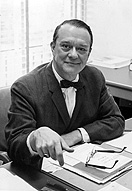
\includegraphics[width=.85\textwidth]{figures/Smith.jpg}
  \caption{Henry Lee Smith}
  \label{fig:ch.structuralists.smith}
\end{wrapfigure}
George {\Trager} (Figure~\ref{fig:ch.structuralists.trager}) was perhaps
the most radical of those claiming to develop {\Bloomfield}'s thought
directly, especially regarding the rigor (and vigor) with which he
rejected any role for considerations of \isi{meaning} in linguistic analysis
or description. \name{Henry Lee}{Smith} made linguistics visible (or audible)
to the public at large through a popular radio program dealing with
dialect differences in \ili{American English}. He later collaborated with
{\Trager} to produce a standard, if controversial, codification of
phonemic analysis as applied to \ili{English}
\citep{trager.smith51:outline}. Other figures whose work was accepted
as contributing to what became the established position in the field
included \name{Archibald}{Hill}, \name{Martin}{Joos}, and \name{Rulon}{Wells}.

The association among these figures was not merely that of scholars
pursuing the same lines of academic research; it also involved a sense
of personal solidarity and community of interest. Reading the papers
of the time (as well as the commentary in \citealt{joos57:readings}, a
political as much as a scholarly statement), it becomes clear that
they felt themselves to be a group of crusaders with a common
mission. This is of course a perfectly standard state of affairs in
academic life, but it becomes particularly important under the
conditions of American linguistics in the 1940s and early 1950s when
there was no single, dominant personality in the field and when
responsibility for scientific judgment was therefore more than usually
diffused.

A figure whose work was clearly central to the dominant theoretical
trend but who was somewhat outside it in more personal terms, was
\name{Zellig}{Harris}. {\Harris}'s rigorous and purely distributional methods in
linguistic analysis must be regarded as the intellectual high point of
the attempts to develop the logical consequences of the
`Bloomfieldian' position. His papers in phonology and morphology, and
his attempt to extend structuralist methods to syntax, were widely
read, attended to, and cited; but he himself seems to have been less
close personally to the community of American linguists than others
mentioned above. In part, this may result from the fact that he came
to linguistics from a background in Semitic rather than in
\ili{Indo-European} (especially \ili{Germanic} or \ili{English}) or Amerindian
studies. It may also result from his frequently expressed outspoken
admiration for {\Sapir}'s methods, even if he devoted much of his
attention to developing a very different alternative. Finally, factors
of personality (possibly including his intense interest in Zionist
political questions, but not limited to this: {\Harris} had something of
a reputation as un-collegial, illustrated for example by his rejection
of an invitation to speak at the Ninth International Congress of
Linguists (section~\ref{sec:emergence}) in 1962) must have played a
role in setting him apart.

Somewhat more marginal was a group of scholars identified as the
successors of {\Sapir} rather than of {\Bloomfield}. These included Morris
{\Swadesh}, Mary {\Haas}, Stanley {\Newman}, \name{Carl}{Voegelin}, \name{Murray}{Emeneau}, and
others with interests oriented more toward anthropological and
Amerindian studies than toward `theoretical linguistics' in the sense
that notion came to have. Those whose sympathies went with {\Sapir} were
evidently more interested in finding accommodation with the
Bloomfieldians than \emph{vice versa}. There is little attempt on
these scholars' part to downgrade {\Bloomfield}'s work, while {\Sapir}'s
views (especially on the \isi{psychological basis of language}) were often
attacked or even derided from the orthodox `Bloomfieldian'
perspective, lumped together with other examples of now \emph{démodé}
`\isi{mentalism}'.

\begin{wrapfigure}{r}{.3\textwidth}
  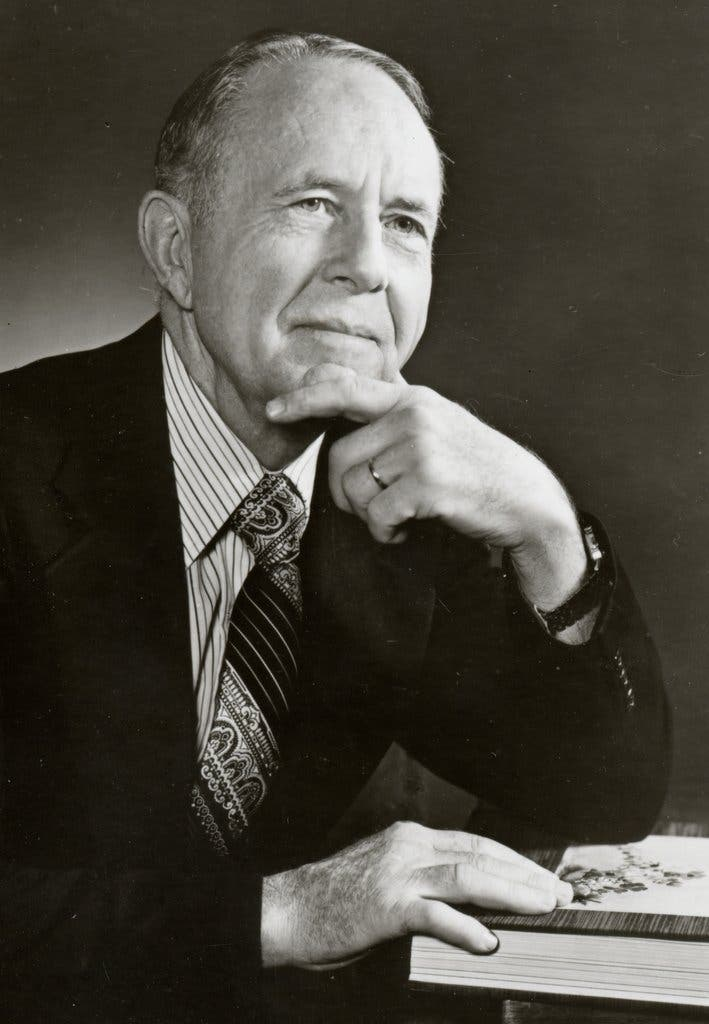
\includegraphics[width=.85\textwidth]{figures/Nida.jpg}
  \caption{Eugene Nida}
  \label{fig:ch.structuralists.nida}
\end{wrapfigure}
Finally, one can identify a group of linguists whose main contribution
to the theoretical debates of American \isi{structuralism} was as
critics. Two of these, \name{Eugene}{Nida} and \name{Kenneth L.}{Pike}, were involved
primarily in the development of practical methods for investigating
unfamiliar languages: in both cases, this concern arose from their
association with the work of Bible translation groups. Another figure,
\name{Charles}{Fries}, shared with {\Pike} a location at the University of
Michigan, but was primarily interested in \ili{English}. All three were
identified as antagonistic toward certain aspects of `Bloomfieldian'
practice— especially the (often overstated) rejection of appeals to
\isi{meaning} in any form.

It is quite interesting to note not only the points on which they
attacked other American structuralists, but also the extent to which
even these critics of the theory shared many of its basic
assumptions. Undoubtedly their position outside the main currents of
the time (as indicated by the freedom with which their views are
attacked or simply rejected by other, more central figures) resulted
from their critical stance, but the more social factor of the lack of
prestige of religiously motivated fieldwork cannot be ignored, at
least in the case of {\Pike} and {\Nida}. The exclusion of any of {\Pike}'s
work from \posscitet{joos57:readings}
collection\footnote{\citet{newmeyer19:joos.readings} recounts some of
  the history involved in the formation of this set of canonical texts
  of American Structuralism.}  is particularly striking, and
impossible to account for in terms either of its intellectual quality
or its relevance to the dominant issues in American structuralist
discussions.

\section{The American structuralist view of language}

Given the number and diversity of the participants in the development
of \isi{American structuralism}, one would hardly expect a single uniform
and homogeneous theoretical position to have resulted from their
work. In hindsight, however, it is also easy to exaggerate the
diversity of this group. While their views naturally evolved over
time, it is impossible to deny the existence of a fundamental
community of opinion among them. Sources for their opinions on
foundational issues are to be sought in the relation they felt existed
between their work and that of earlier traditions, especially in
America.

An important study of the bases of \isi{American structuralism} in previous
work (as it was perceived) is provided by \citet{teeter64:triviality},
who points out some important basic assumptions and their
sources. First, from {\Boas}'s \isi{stress} on the individuality of linguistic
systems, and the necessity to consider each system in its own right,
the notion was taken over that there are no universally valid
structural principles in language.  I have argued above
(chapter~\ref{ch.boas}) that {\Boas} did not at all deny the existence of
linguistic \isi{universals}: indeed, his notion of language structure was
based on rather strong assumptions not only about the form of
grammars, but also about the substantive content of both semantics and
phonetics. Nonetheless, his emphasis on diversity (intended to combat
the traditional \ili{Latin}-based grammatical model) was interpreted as a
demonstration that ``languages could differ from each other without
limit and in unpredictable ways,'' in the much-cited formulation of
\citet[96]{joos57:readings}

{\Joos}'s remark was aimed explicitly at the sort of phonological
theory developed by {\Trubetzkoy} and {\Jakobson}, based as it was on the
assumption of a universal set of phonological features and the search
for far-reaching universal principles of phonological
systems. Nonetheless, the scope of the objection is broader than
this. {\Boas} is also cited, for instance, as the ultimate source of
potential skepticism about the validity of even a phonetic
\isi{segmentation} of the speech signal: from him, the ``practicing linguist,
in the American sense'' had learned that in this respect too ``[i]n his
{\Boas} tradition (languages can differ without limit as to extent and
direction), no universal theory of segments can be called on to settle
the moot points. Only the particular language can yield proper
criteria. Where these fail, \isi{segmentation} is arbitrary.''
\citep[228]{joos57:readings}.

\begin{wrapfigure}[11]{r}{.25\textwidth}
  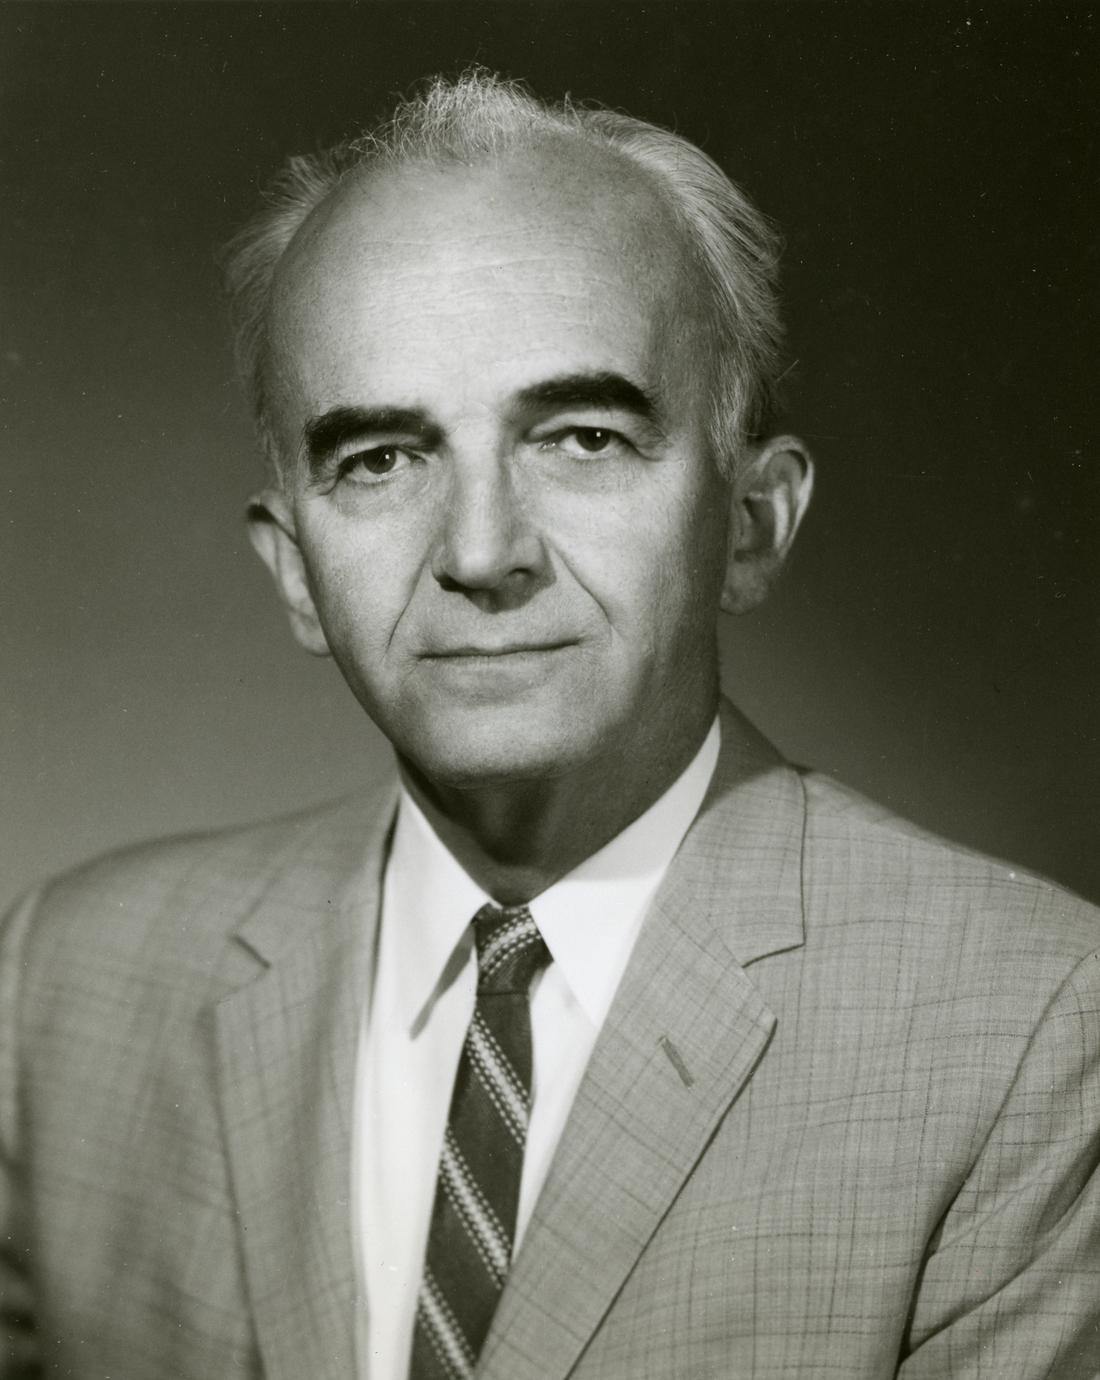
\includegraphics[width=.85\textwidth]{figures/Joos.jpg}
  \caption{Martin Joos}
  \label{fig:ch.structuralists.joos}
\end{wrapfigure}
The claim that linguistics could not successfully be based on a search
for valid \isi{universals} of language was considered by {\Joos} as a
conclusion from {\Boas}'s work that might have to be reexamined. ``The
abandonment of \isi{deduction} in favor of induction has never been
reversed. At first it left the science stripped of general doctrines
about all languages. Favorable at the start, this state of opinion
could be, and in many older workers actually was, maintained past its
function and could become a hindrance to further development. Once a
number of unprejudiced descriptions had resulted from it, induction
could be applied to those new descriptions too, and general doctrines
about all languages could emerge again''
\citep[v]{joos57:readings}. The problem with a program such as that of
the Prague school, then, was not the simple fact of looking for
\isi{universals} but the attempt to present a deductive, explanatory
system. Universals should, rather, be discovered as purely inductive
generalizations.

This is a point with profound implications for the sort of work
linguists should do. If they believe there is a general set of
explanatory principles underlying language, and that it is their goal
to find and understand these principles, they ought presumably to
organize their work by formulating tentative systems with a rich
deductive structure, and then look for evidence of the fit between
such systems and the properties of actual natural languages. {\Joos}
indeed attributes a related motivation to {\Boas} as well: ``A general
truth about language, to {\Boas}' way of thinking (or perhaps feeling),
would have to be based on nothing less than the biological or even the
physiological character of man (he was a physical anthropologist too)''
\citep[v]{joos57:readings}. One wonders at the omission of the
psychological character of man, as well, given {\Boas}'s intense interest
in human mental life; but in any event {\Joos}'s objection to {\Boas}'s
presumed \isi{deduction} of the properties of natural languages from a
limited set of foundational assumptions is that while an explanatory
system of principles might be possible, it would have to be based on
factors outside of language, and any ``such theories still lay far in
the future''.

Recognition of the limitations on how far linguistics could go in
making connections with the only apparently possible bases for an
explanatory theory (i.e., with extra-linguistic factors) was attributed
to {\Bloomfield}. {\Bloomfield} was generally held to have insisted that
linguistics must proceed without reference to the mind, a restriction
that not only prevented theorizing about the psychological
implementation of linguistic structure but, indeed, eliminated all
serious work in semantics. It will be recalled (from
chapter~\ref{ch.bloomfield}) that what {\Bloomfield} actually maintained
was not so much the nonexistence of mind as its inaccessibility to a
physicalist theory in the absence of comprehensive, encyclopedic
knowledge from other domains; but in practice the two were the
same. While {\Boas} had undoubtedly believed that psychological
explanations would be forthcoming for many aspects of linguistic
structure, the narrow interpretation of {\Bloomfield}'s views about
psychology ruled out the possibility that such a basis could be found
for explanatory principles underlying the nature of language.

Similarly, {\Bloomfield} had argued that phonetic data (apart from the
implementation of phonemic contrasts) were simply irrelevant to
linguistic structure. This view was based on the claim that, from the
perspective of a given language, phonetic facts other than contrastive
ones were more or less accidental concomitants of the distinctive
properties. Of course, fieldworkers no more abstained in practice from
the use of \isi{phonetic representations} and assumptions than {\Bloomfield}
had done in his own fieldwork; but his rejection of theoretical status
for phonetics within linguistics was widely quoted with approval.

\begin{wrapfigure}[11]{r}{.4\textwidth}
  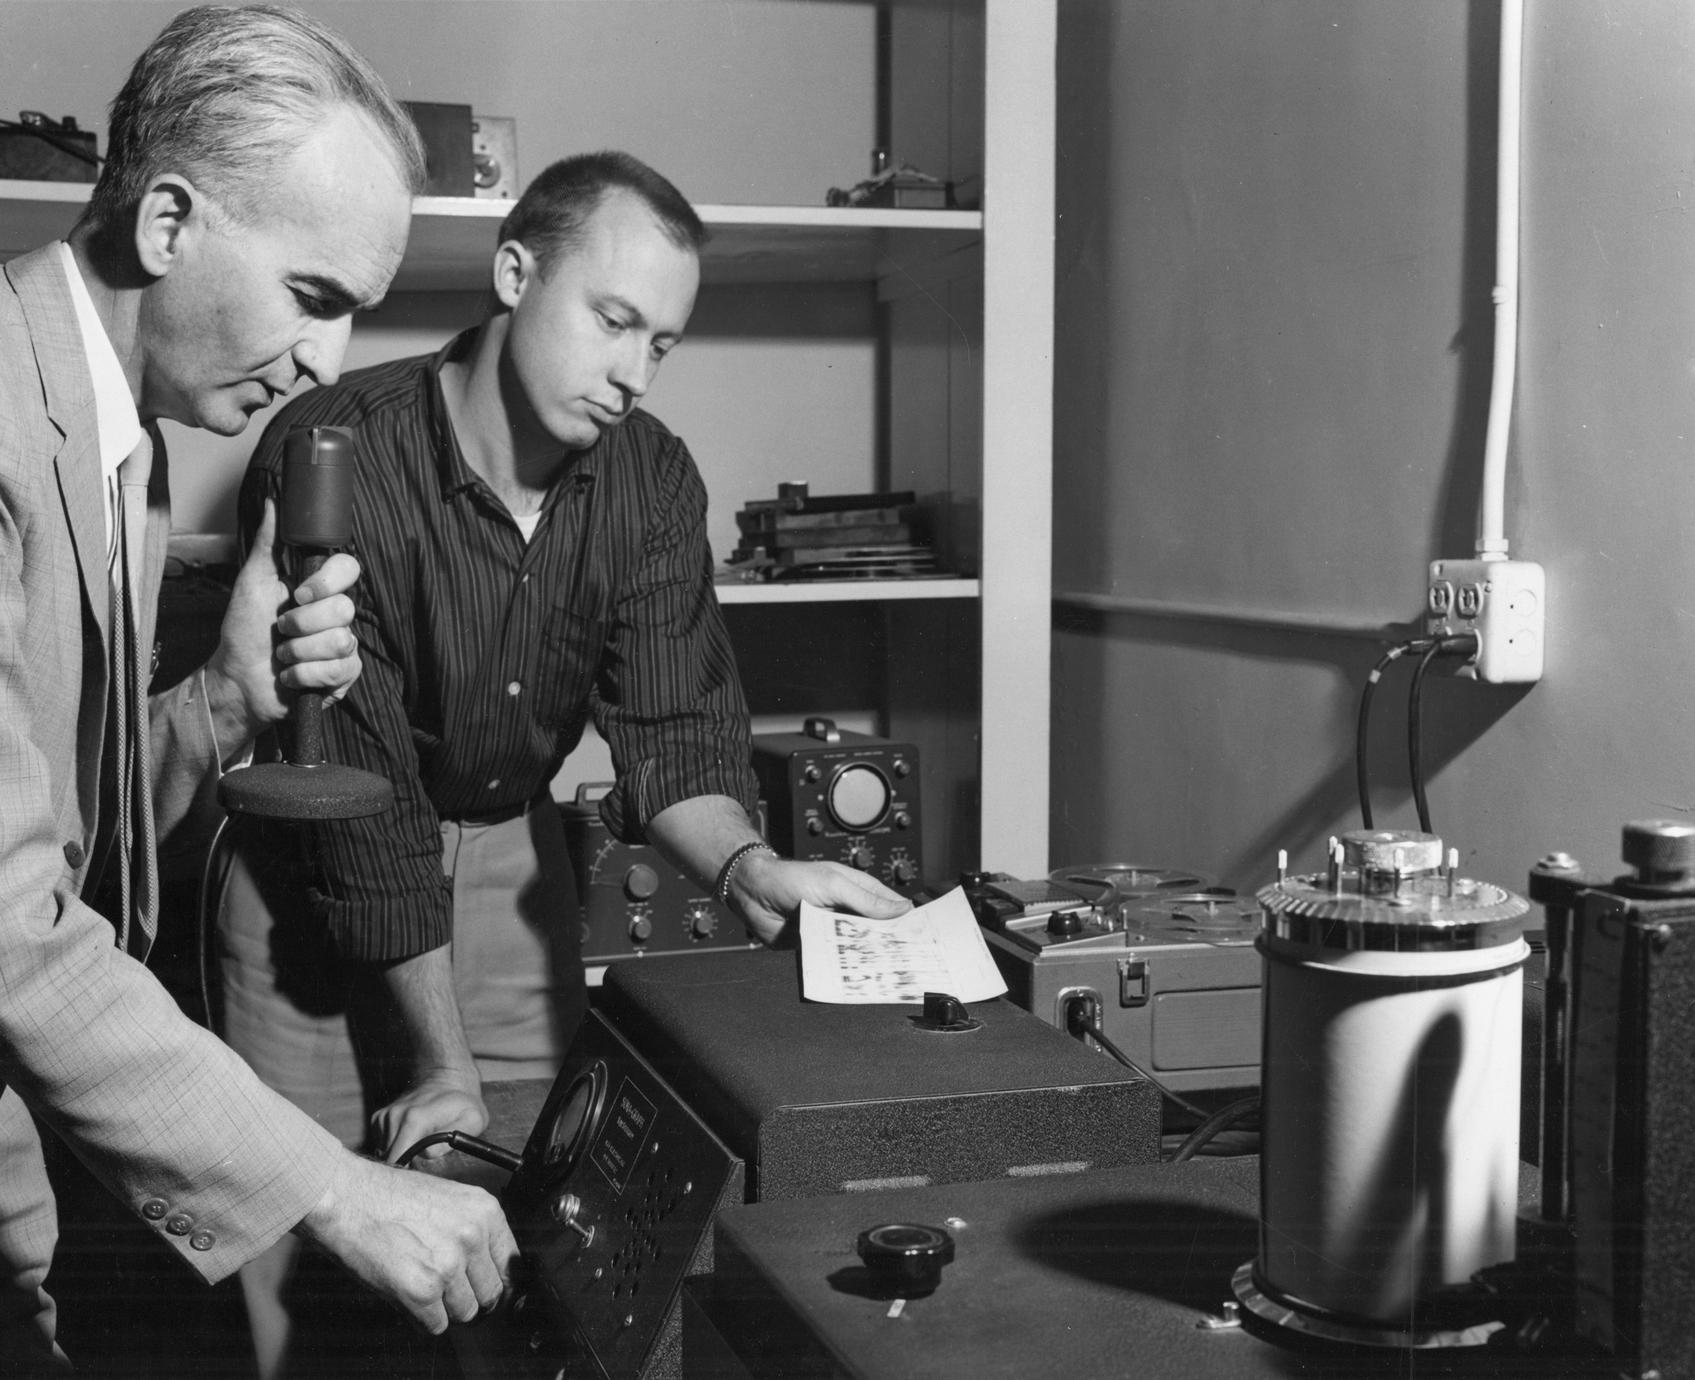
\includegraphics[width=.85\textwidth]{figures/Joos-phonetics.jpg}
  \caption{Martin Joos engaged in early acoustic phonetic research}
  \label{fig:ch.structuralists.joos-phonetics}
\end{wrapfigure}
In the absence of a serious notion of universal phonetics (apart from
physics and physiology, non-linguistic disciplines treating the facts
of language without distinguishing them from others), there was simply
no way for phonetic data to serve as the foundation of linguistic
explanations. Interestingly, both \citet{pike43:phonetics} and
\citet{hockett55:manual} wrote full-scale treatments of phonetics, and
\citet{joos48:acoustics} presented the first systematic exposition of
the application of the techniques of acoustic analysis to linguistic
phonetics. Nonetheless, in the theoretical literature the status of
phonetics remained (in principle) that of an auxiliary
discipline. Though it was \citet{trubetzkoy39:grundzuge}---crediting
{\Jakobson}---who was responsible for the aphorism that ``phonetics is to
linguistics as numismatics is to economics,'' the attitude was the same
among American structuralists. Linguistics was thus cut off on both
sides (semantics and phonetics) from any access to principles that
could have a possible explanatory role.

Since the only valid roads to a deductive theory of language were thus
(at least temporarily) foreclosed, the only acceptable activity for
linguists in the meantime was the neutral gathering of facts about as
many languages as possible; and the only acceptable `general
principles' of language were inductive generalizations based on the
available corpus of such descriptions. This reasoning led to a
widespread replacement of \emph{structural} as an epithet for
linguistics in America by \emph{descriptive}, to emphasize the fact
that the primary task was conceived of as the gathering of unbiased
information rather than the supposedly premature search for
explanatory principles.

In the work of American structuralist (or, as they preferred to call
themselves, descriptive) linguists, these general principles led to a
number of rather well-marked characteristics. For example, it is
obvious that these notions would further emphasize the tendency in
American linguistics (already strong, as a result of its
anthropological and Amerindianist origins) to concentrate on extensive
fieldwork. In the absence of deductive explanatory principles, the
only scientifically respectable activity for linguists was to go on
looking at as many languages as possible. Of course, linguists other
than American structuralists also made it a point to seek out data
from a wide range of languages: {\Trubetzkoy} and {\Jakobson}, for example,
can hardly be faulted for not paying attention to such
considerations. Nowhere else, however, did description for its own
sake acquire the prestige among linguistic scholars that it had in
America during the structuralist period.

This bias hardly prevented the writing of papers whose primary thrust
was theoretical in nature; but it did contribute to the establishment
of a `standard form' for such papers, in which the theoretical point
is presented in the context of a discussion of specific facts and how
to `handle' them, rather than exclusively on its own account. This is
a characteristic of American linguistic writing which continues
largely unabated today, and which still distinguishes it from much
European work in linguistic theory.

Another observable emphasis in American descriptive work was the
concern to remain within the bounds of what was considered
`scientific'. In the context of the positivist, mechanist,
operationalist, etc., views current in the philosophy of science at
the time, this meant avoiding appeals to unobservable factors (`mind',
`intuitions', etc.) in description. Especially important was the
requirement that analyses had to be replicable, in the sense that any
observer, given the same data and a mechanical statement of the way
analyses were to be arrived at, would be able to come up with the same
account. Analyses based on the investigator's intuitions about the
structure of the language, unless these could be translated into
manipulations of observable data, were thus invalid.

A natural consequence of this need to make the description
sufficiently explicit to be replicable was a tremendous concentration
(at least on the part of `orthodox (neo-)Bloomfieldians' such as
{\Bloch}, {\Harris}, and their close associates) on specifying procedures of
analysis. This concern might also be seen as arising from the fact
that in the absence of underlying explanatory systems, the procedures
by which linguists reduced data to descriptions of language were
virtually the only subject matter of linguistics that remained to talk
about; but this would not be at all the entire story.

Many subsequent writers on the period have suggested that it was
characterized by a general lack of `theory'; but that is to miss the
importance of the description of analytic procedures. Some field
workers, of course, were primarily interested in describing actual,
practical procedures to be followed by a linguist working on an
unfamiliar language from scratch; but such concerns were not really
what was meant by the concern with analytic procedures in the
literature of the period. Most theoreticians realized (generally from
firsthand experience) that fieldwork involved repeated access to
intuitions, guesses, shortcuts, appeals to \isi{meaning}, etc.; but it was
still required that an analysis be validated by specifying a
mechanical procedure that could, in principle, have been followed so
as to lead inexorably from observations to the resulting description
without the intervention of unsystematic factors. Such a
`\emph{gedanken}-experimental' reconstruction of the connection
between data and analysis, no matter how tortured and impractical
under real conditions, served to establish the point of principle that
no unobservable or un-replicable factors were involved in an essential
way.

It is difficult to exaggerate the extent to which this concern with
the explicit formulation of (at least theoretically applicable)
procedures dominated the style of linguistic work in the American
structuralist period. The present writer, whose initial studies in
linguistics were with representatives of this approach, recalls
vividly a succession of arguments from one of his teachers whose essential point was: ``I don't
care if it is the `right' answer; how do you justify having found it?''
Linguistic theory, in the absence of \isi{universals} or an appeal to
underlying explanatory principles, was by no means nonexistent; but it
did reduce largely to the specification of what connection existed
between facts of language and their analysis. This connection was to
be formulated in terms of a set of procedures (most extensively and
rigorously by \citet{harris:methods}; but the aim was shared by most
workers in the field). As a result, linguistics found itself in the
curious position of appearing to have much more to say about the
activities of linguists than of speakers of natural languages.

This seemed perfectly natural at the time, however, especially in the
context of available theories of the learning that was presumed to
underlie language acquisition. If we assume that the child comes to
the language-learning task with the same absence of presuppositions
that the linguist was trying strenuously to achieve, it is natural to
imagine that their paths to language are much the same. If
language-learning proceeds along a purely inductive path, without
recourse to assumptions or unobservable factors, the same sort of
procedures followed (at least in principle) by the hypothetical field
linguist ought to specify what results. But in that case, the class of
languages accessible to the child (the class of possible natural
languages) is adequately and accurately specified by the description
of the procedures that could possibly be involved in their acquisition
from primary linguistic data.

In a paper considered at the time to be an outspoken defense of the
`reality' of linguistic structure as opposed to the notion that
linguistic analysis is simply a matter of playing games with language
data, \citet{hockett48:structure} made it clear that he saw an
essential similarity between the activities of the linguist and of the
child: ``The analytical process thus parallels what goes on in the
nervous system of a language-learner, particularly, perhaps, that of a
child learning his first language \ldots\ The essential difference
between the process in the child and the procedure of the linguist is
this: the linguist has to make his analysis overtly, in communicable
form, in the shape of a set of statements which can be understood by
any properly trained person, who in turn can predict utterances not
yet observed with the same degree of accuracy as can the original
analyst. The child's `analysis' consists, on the other hand, of a mass
of varying synaptic potentials in his central nervous system. The
child in time comes to behave the language; the linguist must come to
state it.'' Though such a strongly `realist' position on the nature of
linguistic structure was probably a minority one, for those who took
it, such a presumed parallel between the linguist and the child could
be seen to validate the formulation of analytic procedures as a
genuine theory of natural language.

Another, related assumption should also be mentioned as relevant to an
understanding of the specific linguistic theories developed by
American structuralists. It was generally assumed that, like the
learning system, the perceptual system of human speakers of natural
languages operated with little or no access to facts beyond the
immediately observable. In particular, it was generally taken for
granted that the `outer layer' of \isi{speech perception} was a system that
takes an acoustic waveform as input, and on the basis of nothing but a
specification of the phonemic system of the language, yields as output
an interpretation of that waveform in the form of a sequence of
phonemes. After this initial processing has been performed, `higher'
\isi{levels} of the speech-understanding system can operate on the string of
phonemes to yield an interpretation in terms of morphemes, and so on
up through higher level structures.

If \isi{speech perception} involves such a `bootstrapping' interpreter,
whose operation consists of little or nothing but the \isi{segmentation} and
consequent classification of raw acoustic input, a number of essential
properties of the \isi{linguistic system} follow. In particular, it must be
the case that language involves an essential intermediate level of
structure which is directly recoverable from the speech signal, and
which contains all (and perhaps only) the information relevant for
higher-level interpretation. If only this sort of phonemic level is
accessible in principle to the perceptual system, it follows (at least
on moderately `realist' assumptions about linguistic structure) that
phonemic analyses not meeting such a condition should be excluded in
the description of natural languages. This led to another of the
important slogans of the period: the prohibition against `mixing
\isi{levels}', or allowing considerations from higher \isi{levels} of structure to
play an essential role in determining the relation between phonemic
and \isi{phonetic representations}.

Given the premise that the actual speech signal is much too complex to
be directly manipulated by higher \isi{levels} in speech processing, and
that some sort of phonological representation mediates between the
signal and the analysis of its linguistically relevant properties, it
seemed self-evident that the phonological representation could only
have properties that were recoverable from the bare signal
itself. Only much later, with the development of rather richer and
more highly structured views of perception as an active rather than
purely passive process (along the lines of the `analysis by synthesis'
view, for example: see \citealt{halle.stevens62:analysis.by.synthesis}
for an early proposal), did it become possible to imagine a coherent
picture of phonological structure that transcended these
limitations. Until then, however, it seemed clear to linguists that
what could be assumed with confidence about the process of perception
provided further motivation for a rather minimal theory of linguistic
structure, along the lines of American structuralist phonemics.

\section{Initial formulations of the notion of `phoneme'}

Against this general background, I turn now to the specifically
phonological aspects of American structuralist linguistic theory. On
the basis of the claim by {\Bloomfield} and others that a representation
of the significant sound properties of utterances should take the form
of a sequence of phonemes, the fundamental task for a theory of
phonology was clearly to provide an adequate definition of what
phonemes were.

{\Bloomfield} had given a definition (``minimal same of vocal feature'')
which located phonemes in the external phonetic form of the utterance
as a subset of its identifiable acoustic properties. This concrete
physical definition did not satisfy all analysts,
however. Furthermore, many examples of phonemic analyses in
{\Bloomfield}'s own practice did not seem to be easily reconciled with
his definition, and attempts were made either to reformulate the
notion of \isi{phoneme} so as to be consistent with those analyses, or else
to defend more consistent ones. In this discussion, the type case (as
indicated in the previous chapter) was {\Bloomfield}'s treatment of
reduced vowels—and, by implication, other instances of phonologically
conditioned \isi{neutralization}. The central issue in this discussion
gradually crystallized as the extent to which \isi{phonemic representations}
should be unambiguously recoverable from phonetic data alone.

Discussion of the nature of the \isi{phoneme} became a major topic in the
journals of \isi{American structuralism}. Indeed, {\Bloomfield} is said once to
have suggested to {\Bloch}, as editor of the journal \textsl{Language},
that the number of papers on phonemics was getting to be excessive and
should be reduced. The starting point for many of these discussions
was {\Bloomfield}'s own definition, but virtually none of the subsequent
writers on the topic accepted in detail his notion of the nature of
the \isi{phoneme}. A number of alternative conceptions emerged, gradually
converging on a consensus view by the late 1940s. By that time, the
problem had shifted from what phonemes were to how to define
operational procedures that would yield them.

Shortly after the publication of \citealt{bloomfield:lg}, the issue of
reduced vowels and their implication for phonemics was addressed in
George \posscitet{trager34:russian} article on ``The Phonemes of
\ili{Russian}''. He summarizes the issues raised between {\Bloomfield} and
\citet{kent34:rvw.bloomfield} noted above in chapter 10, and in
particular the difference between {\Bloomfield}'s treatment of vowel
reduction and that of final \isi{consonants} in \ili{Russian}. {\Trager} finds the
disparity between these two parts of the analysis unsatisfactory, and
proposes that an adequate phonemic analysis should be based on the
uniform principle of ``avoid[ing] the use of more than one symbol for
the same sound (except where differing structure permits the
distinction into two phonemes)'' \citep[339]{trager34:russian}

Subject to the qualification in parentheses, this would prevent the
analyst from representing the same phonetic segment (in the same
environment) differently in different words. In the relevant instance,
\ili{Russian} final [t] could not be identified as /t/ in some words (e.g.,
\emph{rot} `mouth') but as /d/ in others (e.g., \emph{rod}
`kind'). However, the issue turns entirely on when ``differing
structure permits the distinction into two phonemes.'' {\Trager} argues
that when there exists an \isi{alternation} between two otherwise distinct
phonemes, conditioned entirely by their phonological environment, and
internal to a paradigm, then ``since the paradigm exists in the mind of
the speaker as a psychological reality, there exists a psychological
difference in the sounds,'' found in the position of \isi{neutralization} as
well \citep[341]{trager34:russian}.

In {contrast}, when there is no intra-paradigmatic \isi{alternation}, the only
available phonemic interpretation is ``complete psychological
identification of the original voiced sound with the new, voiceless
sound, and their merging into the voiceless \isi{phoneme}, despite the
presence of the voiced sound in the original of the derivative, or in
some other derivative'' \citep[342]{trager34:russian}. The similarity
of this condition to the ``Revised Alternation Condition'' proposed by
\citet{kiparsky:3dimensions} in the context of the debate over
\isi{abstractness} in generative phonology will not be missed.

It should be noted that the criterion of phonological conditioning is
intended by {\Trager} to be a necessary one. Where two phonemes alternate
under conditions that are at least partially morphological in nature,
he treats the difference as `morphonemic', and argues that it does not
affect the phonemic representation directly.

It is somewhat ironic that {\Trager}, who would later become one of the
most extreme `anti-mentalists' among the main stream American
structuralists, takes a stand in this article much closer to that of
{\Sapir} than to that of {\Bloomfield}—indeed, he refers explicitly to
\citealt{sapir25:sound.patterns} for the notion of a psychological
difference between `ideal' sounds that happen to be phonetically
identical. This is a reflection of the fact that he was acquainted
with {\Sapir} before he was with {\Bloomfield}.

\begin{wrapfigure}[11]{r}{.35\textwidth}
  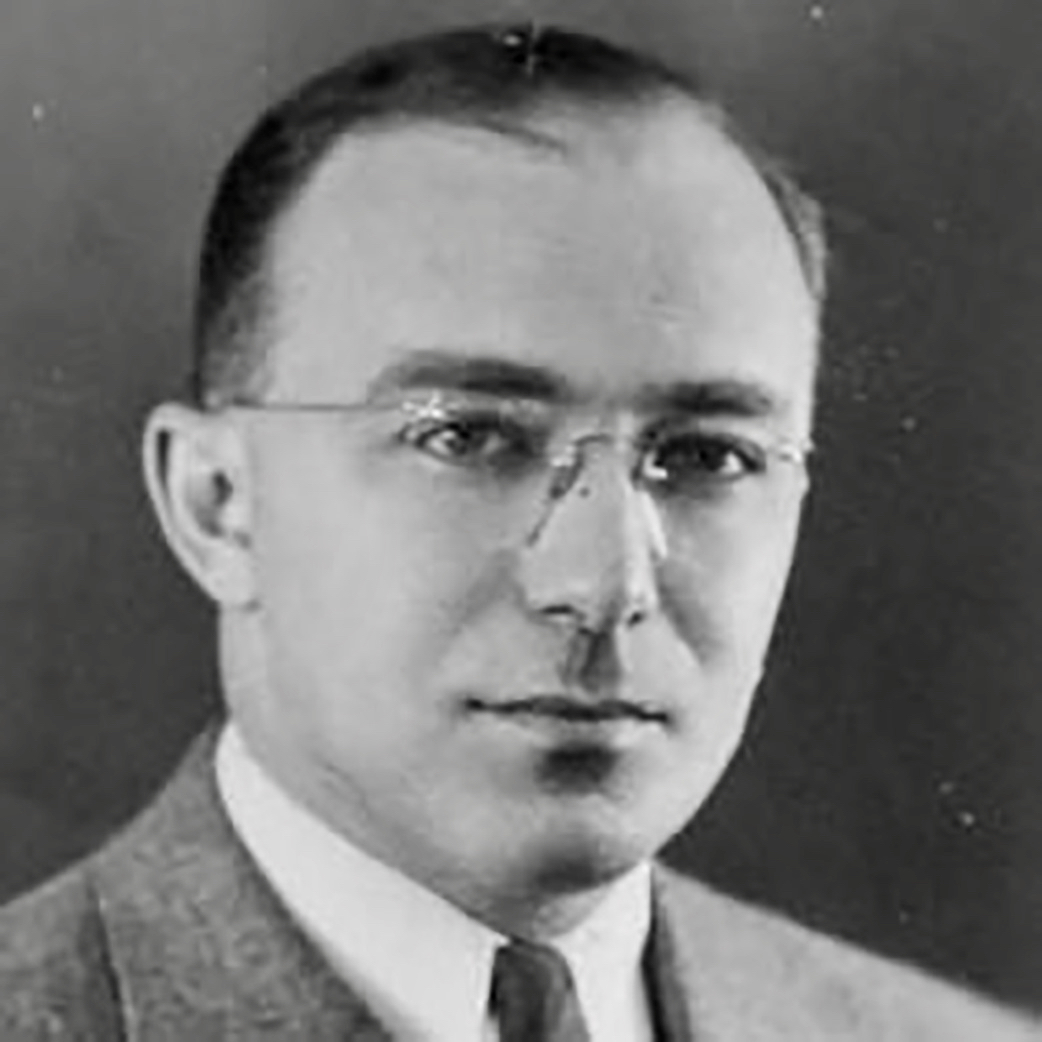
\includegraphics[width=.85\textwidth]{figures/Trager1.jpg}
  \caption{George Trager}
  \label{fig:ch.structuralists.trager}
\end{wrapfigure}
Trager\ia{Trager, George}'s background was in Romance Linguistics at Columbia, where he
had come under {\Boas}' influence (though he was not actually {\Boas}'
student). According to \posscitet{hockett93:trager.obit} obituary, he
probably had some contact with {\Sapir} and with {\Swadesh} even before
1934, and between 1936 and 1943 he was associated in various ways with
the Linguistics Department at Yale, where he would of course have been
in {regular} association with {\Sapir} until the latter's death in
1939. When {\Bloomfield} came to Yale in 1941, they would have naturally
been closer than before, but as a result of various frictions between
them, {\Trager} held a less than cordial attitude toward {\Bloomfield},
according to {\Hockett}.

Personal relations aside, \posscitet{trager34:russian} ``Sapirian''
slant on phonemics was not really an anomaly. As noted in
chapters~\ref{ch.sapir} and~\ref{ch.bloomfield}, {\Sapir}'s influence
(and indeed priority with regard to the notion of the \isi{phoneme}) was
still clearly recognized during the 1930s. {\Bloomfield}'s
\textsl{Language} did not immediately upon publication supersede all
other work.

Such irony as may be found in {\Trager}'s stance is compounded, however,
by the fact that a linguist much more closely identified as {\Sapir}'s
student, Morris \citet{swadesh34:phoneme}, presented in the same
volume of \textsl{Language} a formulation of the basic principles of
phonemic analysis which is much closer to the orthodox `Bloomfieldian'
view. Though {\Swadesh} starts from a position that could be construed as
basically Sapirian (characterizing phonemes as ``percepts,'' and thus
psychological in character), his actual development of the position is
much more external in conception than {\Sapir}'s own discussions.

According to \citet[123]{swadesh34:phoneme}, the ``inductive
procedure,'' which is the only way in which ``the phonemes of a
language can be discovered,'' begins naturally enough with the
phonetic facts. First, it is necessary to normalize the phonetic
material somewhat, by abstracting away from free \isi{variation} so as to
arrive at a consistent representation for each word. One then performs
a phonetic \isi{segmentation}, looking for sub-stretches of words that
establish partial identities between them, and treating as units sets
of phonetic properties that are found in constant association. Two or
more of the resulting phonetic segments can then be treated as
``subtypes of the same \isi{phoneme}'' if they are in complementary
distribution (i.e., ``only one of them normally occurs in certain
phonetic surroundings, and \ldots\ only the other normally occurs in
certain other phonetic surroundings'' (\emph{Ibid})). When
\isi{complementary distribution} would allow the assignment of a given
segment type to either of two possible phonemes, ``it is to be
identified with one rather than the other if there is a more definite
phonetic similarity in that direction'' (\emph{Ibid}). Here, in
essence, is the procedure whose refinement as a definition of
`\isi{phoneme}' would constitute the core of American structuralist
phonology.

\begin{wrapfigure}{l}{.35\textwidth}
  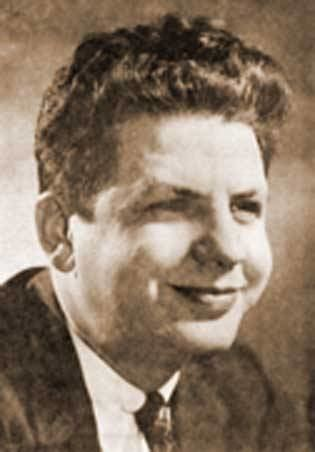
\includegraphics[width=.85\textwidth]{figures/morris-swadesh.jpg}
  \caption{Morris Swadesh}
  \label{fig:ch.structuralists.swadesh}
\end{wrapfigure}
In only one major respect does {\Swadesh} differ from the majority of
later writers: this is the issue of the phonetic substance of
phonemes. As noted above, he considers phonemes to be ``percepts''
identifiable with a phonetic type, where ``it is possible to define
the type in terms of a [phonetic] norm and of deviations from the
norm'' \citep[119]{swadesh34:phoneme}. When more than one phonetic
type is assigned to the same \isi{phoneme} (by virtue of their
complementarity of distribution), ``instead of one norm, there may be
two or more. Such variant norms are ordinarily conditional, depending
on the phonetic surroundings in which the \isi{phoneme} occurs''
(\emph{Ibid}). The \isi{phoneme} itself is thus defined by an ideal phonetic
segment type, as for {\Sapir}; {\Swadesh}'s notion of phonological
representation is fundamentally a `completely specified basic variant'
theory as defined in chapter~\ref{ch.saussure_sound} above, but
differs from, for example, {\Sapir}'s version of this position by
allowing more than one `basic variant' for the same \isi{phoneme}. Others
would take this one step further, by identifying the \isi{phoneme} not with
any of its phonetic variants (`ideal' or not), but rather with the
class constituted by their union.

It is important to note that {\Swadesh}'s procedure (which is said to
``follow from the nature of the \isi{phoneme}'',
\citealt[123]{swadesh34:phoneme}) allows no possibility of phonemic
differences that are not recoverable from the phonetic facts. In fact,
he does not discuss any potential examples of this, and we do not have
direct evidence in this paper for the way he would have treated
them. Given his association with the tradition of {\Sapir}, and his
practice in later work, we can presume that he would have wanted to
recognize `psychological' differences in the phonemic value of the
same phonetic segment as it appears in different words (depending on
such evidence as alternations); but his actual statements make no
provision for this situation, and therefore appear to preclude it. The
general circulation and accessibility of {\Swadesh}'s paper may thus have
contributed to reinforcing in practice an attitude toward phonemics
which was more physicalist than he in fact intended.

{\Swadesh} also discusses, in treating the establishment of the phonemes
of a language, the ways in which a set of phonemes are organized into
a system. Indeed, he establishes a requirement that phonemic analyses
should be established so as to maximize `\isi{pattern congruity}'. This
notion was to be interpreted as the integration of particular details
into ``the general phonemic pattern of the given language''
\citep[124]{swadesh34:phoneme}.

The establishment of systems (rather than simply inventories) of the
pho\-nemes of a language was a task which most American structuralists
recognized as part of the task of phonological theory, though such a
goal is somewhat difficult to understand on purely internal
grounds. For most, the role of phonemes in linguistic structure was
the purely differentiating one of identifying the distinctive function
of sound units, and little else. Internal relations (beyond mere
mutual distinctness) among the phonemes of a given language were the
subject of much discussion, but it is hard to see what role these
relations played, once established. American structuralists did not,
for example, attempt to establish general structural laws of
phonological systems based on their internal organization, as did
{\Trubetzkoy} and {\Jakobson}. One must apparently assume that the
attribution of structure to \isi{phoneme} systems in this view was simply
unconnected with other aspects of the theory.

{\Sapir} and {\Bloomfield}, it may be recalled, had also discussed the bases
for assigning a structure to the system of phonemes in a
language. Both had denied a constitutive role in such structures to
phonetic similarity \emph{per se}; {\Swadesh}, however, in line with the more
physicalist form of his theory, admits phonetic properties as at least
contributory to phonemic structure. Likewise, many would add as a
desideratum for phonological systems a tendency to symmetry along the
phonetic dimensions of \isi{contrast}. This can also be expressed as the
claim that it is most natural for the various features which serve to
distinguish one \isi{phoneme} from another within a language to be
independently distributed among the phonemes.

In addition to these factors, however, {\Swadesh} and other writers admit
further criteria under the notion of `\isi{pattern congruity}'. Some are
common to earlier work: segments that share distributional properties
are assumed to be \emph{ipso facto} similar, for example, as claimed
by both {\Sapir} and {\Bloomfield}. In addition, phonemes whose internal
distribution of phonetic variants follow similar principles (e.g., all
of the voiceless \isi{stops} in \ili{English} have aspirated, unaspirated, and
unreleased variants under essentially the same conditions) were
considered to be thereby related. Further, segments which were related
by \isi{alternation} were considered by some (following {\Sapir}, but not
{\Bloomfield}) to be related to each other within the system by virtue of
this fact. `Pattern congruity' involved maximizing all of these forms
of relatedness among phonemes.

All of these factors contributing to the internal structure of
phonemic systems correspond to \isi{regularities} that, on other theories,
would be treated as rules rather than as part of the definition of
units. The character of American structuralist discussion, however,
was such that the burden of such \isi{regularities} was displaced onto the
ontological status of the phonemes themselves. Of course, linguists
stated \isi{regularities} of distribution when they found them. Such
statements were construed, however, not as having independent
importance but as defining the phonemic units. Actual statements of
distribution quite often took the form of mere lists of the occurring
consonant clusters in various positions, arranged perhaps in tabular
fashion for ease of reference but with little or no attempt to extract
generalizations. The \isi{regularities} themselves, and the forms they might
take if construed as rules of the language, were of only incidental
interest: the focus of attention was on the phonemes and their
definitions, which were assumed to constitute the essence of a
language's \isi{phonological system}. We return to this issue and some of
its effects in a later section.

\section{Twaddell's ``On Defining the Phoneme''}
\label{sec:twaddell}

Already by the mid-1930s, then, two distinct conceptions of the nature
of the \isi{phoneme} had emerged within American linguistics. According to
one of these, associated in America with the tradition of {\Sapir} and
elsewhere with such writers as {\DeCourtenay} and {\Trubetzkoy}
(at least in his early work), phonemes were fundamentally
psychological in nature: `ideal sounds', `the mental equivalent of a
\isi{speech sound}', `percepts', etc. In {contrast}, an opposing view
identified with {\Bloomfield}'s definition and also with those proposed
by writers in the British tradition such as \name{Daniel}{Jones}, considered
phonemes to be overt aspects of the physical speech event: either some
constant fraction of the phonetic properties of sounds identified as
functionally equivalent; or as classes of actual, fully specified
sounds that are so identified. A monograph by W. Freeman
\citet{twaddell35:on.defining} challenged both of these positions and
suggested that `phonemes' are simply fictitious units used in order to
express an analysis of the contrasts in a language as a system for
transcribing utterances in that language.

\begin{wrapfigure}{r}{.6\textwidth}
  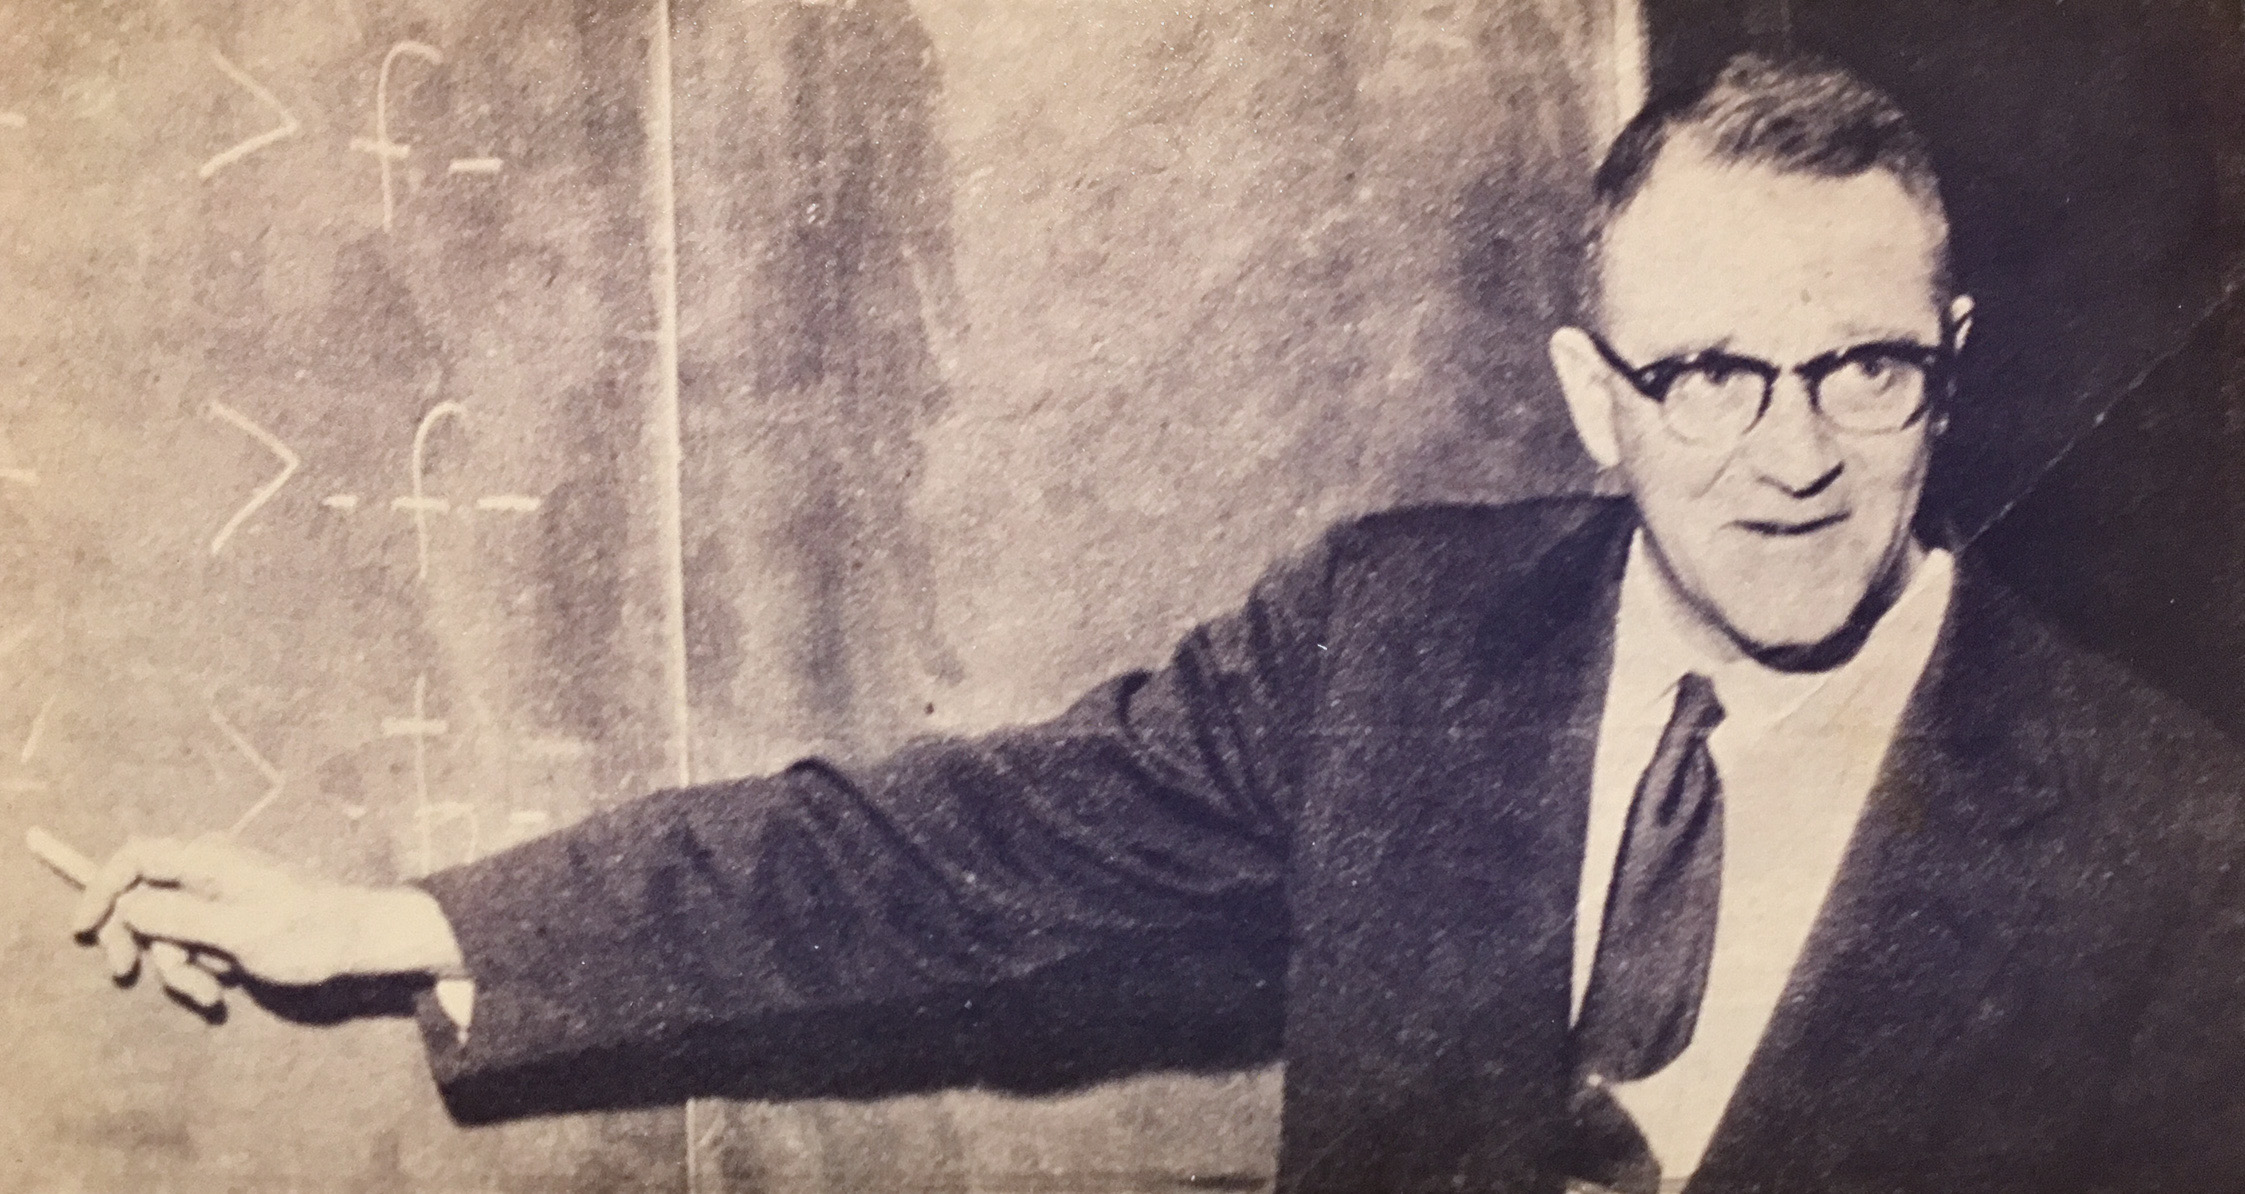
\includegraphics[width=.85\textwidth]{figures/Twaddell_1.jpg}
  \caption{W. Freeman Twaddell}
  \label{fig:ch.structuralists.twaddell}
\end{wrapfigure}
Twaddell\ia{Twaddell, W. Freemen} attacks the psychological view of the pho\-neme first, in
terms heavily dependent on {\Bloomfield}'s view of psychology. Since on
that view we know nothing at all about the `mind' except what we can
observe externally in terms of stimuli and responses, it is a
conceptual and logical error to say that phonemes are a `mental'
reality. For {\Twaddell}, as for {\Bloomfield}, such descriptions simply
assign a name to the unobservable: ``they identify an entity which is
inaccessible to scientific methods within the frame of linguistic
study''\citet[9]{twaddell35:on.defining}.

\largerpage
{\Twaddell} considers the arguments of
\citet{sapir25:sound.patterns,sapir33:reality} in some detail. He
reviews the several examples reported by {\Sapir} in which speakers
characterized objectively different sounds in the same way (from which
he had argued that the sounds in question corresponded to the same
`mental reality'), as well as those in which speakers characterized as
different sounds that are phonetically the same. In the former cases,
{\Twaddell} argues that all that is involved is the informant's failure
to make some distinction which a trained phonetician might make, and
that the examples thus provide no evidence at all for a non-overt,
`mental' reality. In the second group of {\Sapir}'s examples, {\Twaddell}
argues that the differences being characterized are morphological
rather than phonological in character. While they attest to a
speaker's ability to distinguish morphological or lexical classes,
they do not therefore bear on the claim of a `mental' difference in
\isi{phonemic representations}, because there is no evidence that the
distinction in question is fundamentally phonological and not simply a
matter of differential responses given to different morphological
categories.

The position {\Twaddell} defends in the face of {\Sapir}'s examples is
difficult to argue against on empirical grounds. On the one hand, he
claims that where speakers fail to distinguish phonetically distinct
sounds, that is simply a fact to be registered (rather than attempting
to explain why some distinctions, and not others, are made). On the
other hand, when speakers find a difference between forms that the
phonetician cannot distinguish, either there is no other factor
correlated with the difference in question (in which case, there is no
confirmation of the claim of a difference), or there is such another
factor, in which case {\Twaddell} claims that it is this non-phonological
factor, rather than a mentally real phonological difference, that is
at issue. This position, that ``what you see is all you get,'' might
be argued to yield a less-than-satisfying account of many phenomena,
but it is at least internally consistent. Until fundamental critiques
of various forms of behaviorist psychology were developed (in
particular \posscitet{chomsky59:review_skinner} important review of
these views with regard to language), there were few specific
arguments available which would convince such `anti-mentalists' of the
utility of abandoning that stand.

Having excluded (on his assumptions) the psychological view of
phonemes, {\Twaddell} moves on to attack the physicalist views. He
considers first the position maintained by {\Bloomfield}, that phonemes
correspond to \isi{invariant} sub-portions of the phonetic signal. Now a
major advance of early twentieth-century science (including, of
course, phonetics) had been the recognition that the physical world is
essentially continuous, and that no two events are identical in the
sense that a sufficient degree of precision in measurement could not
fail to find a difference between them. As a result of this pervasive
non-identity of phenomena, the problem of discovering actual
invariants across classes of events is a nontrivial one. Certainly
phoneticians had not succeeded in isolating such invariants in the
acoustic (or physiological) record of speech, and {\Twaddell} suggests
that {\Bloomfield} was in error in assuming that these would eventually
be found. He concludes, then, that this first version of the physical
theory of phonemes is at best a program of research for phoneticians,
and not a satisfactory basis for a theory of phonology.

He then moves on to consider the other common variant of the
physicalist view, that of \name{Daniel}{Jones}, that a \isi{phoneme} is ``a family
of sounds in a given language, which are related in character and are
such that no one of them ever occurs in the same surroundings as any
other in words'' (quoted in
\citealt[25]{twaddell35:on.defining}). Against this view, he argues not
that the notions involved are ill defined but, rather, that the
procedure of grouping sounds together on the basis of complementary
distribution is arbitrary.

In positions where certain distinctions are neutralized, that is, it
is required to assign the sounds that \emph{do} occur to phonemes that
also occur elsewhere; and there is no available criterion to validate
one assignment over another. He considers the case of \ili{English} \isi{stops}
after [s] as an example, where {\Swadesh} had argued for assignment to
the voiceless phonemes /p/, /t/, /k/ on the basis of complementary
distribution and phonetic similarity. {\Twaddell} suggests that there are
as many phonetic properties warranting an assignment to /b/, /d/, /g/
as to /p/, /t/, /k/; and that there is accordingly no reason to prefer
one analysis over the other. In the absence of some constant
characteristic distinguishing the sounds of one family from those of
another (which brings us back to the problem with {\Bloomfield}'s view),
the families involved have no unique identifiability and thus no
demonstrable reality.

Having argued that phonemes could not be adequately defined either in
psychological or in purely physical terms, {\Twaddell} suggests that the
appropriate conclusion to draw is that `phonemes' in the sense of
minimal units of distinctive sound function, forming a unitary
inventory within a language and concatenated with one another in an
additive way to form words, are at most a fictional by-product of an
analysis of the distinctive relations within a language. He proceeds
to develop this alternative view, starting from the observation that
words (not segments) are the minimal free forms of a language which
stand in \isi{contrast}. While we can localize the various aspects of a
\isi{contrast} between words in distinguishable segments, we have no \emph{a
  priori} right to identify the contrasts we find in one location with
those found in another. He suggests \citep[34]{twaddell35:on.defining}
that a similar view can be attributed to {\Jespersen} as the basis of
that linguist's lack of enthusiasm for phonemic theories.

{\Twaddell}'s procedure, which resembles in some ways {\Martinet}'s 
notion of `commutation' (section~\ref{sec:functional-phonetics} above) 
begins by registering the minimal contrasts in
every possible environment. The vocalic contrasts among \emph{beet},
\emph{bit}, \emph{bait}, \emph{bet}, \emph{bat}, for example,
constitute one such set; those among \emph{seek}, \emph{sick},
\emph{sake}, \emph{sec}, and \emph{sack} constitute another, etc. In
each set, the primary fact is the array of differences between the
forms taken pairwise; secondarily, we can identify the terms of these
relations of difference—i.e., the phonetic segments which are
different—and call these \textsc{micro-phonemes}. We can then, in each
such set, arrange the differences in some order corresponding to the
phonetic distinctions involved. The sets just mentioned, for instance,
could be ordered by the difference in tongue height in their medial
segments. The order assigned to each such class is effectively
arbitrary, so long as its phonetic basis is stated.

Such ordered classes of minimal differences can then be compared with
each other. In some cases, it is possible to assign orders to two
classes and align them with one another so that ``the qualitative
articulatory differences among the corresponding phonetic events are
similar and in a one-to-one relation''
\citep[38]{twaddell35:on.defining}. For example, the two sets cited
above, ordered by tongue height as suggested, can be so aligned. Given
such a correspondence, ``the sum of all similarly ordered terms
(micro-phonemes) of similar minimum phonological differences among
forms is called a \textsc{macro-phoneme}''
\citep[35]{twaddell35:on.defining}. This process does not rest on a
claim of phonetic identity (even partial) among the micro-phonemes
that are summed in a single macro-\isi{phoneme}, but rather on the fact that
the differences between corresponding members are parallel to one
another.

The set of macro-phonemes of a language will in general be much larger
than the set of `phonemes' in traditional terms, because whenever
there is a different number of contrasts in one position than in
another, the \isi{contrast} sets cannot be put into one-to-one
correspondence, and consequently their micro-phonemes cannot be
identified under macro-phonemes. For {\Twaddell} this was not a
particularly unfortunate result, since it has the merit of not
falsifying the facts. If it is the relations between forms that are
phonologically primary, and there are fewer contrasts in one position
than in another, it is a distortion to make any identification of the
terms of the one set of contrasts with those of the other. His
position here is essentially the same as that of {\Firth}
(chapter~\ref{ch.firth}) on the same issue.

{\Twaddell}'s view thus is fundamentally similar to that which we
attributed to {\Saussure} in chapter~\ref{ch.saussure_sound}: a
phonological theory based on `fully specified surface variants', in
which the substance of the phonology consists in a direct analysis of
the contrasts among surface phonetic segments in various positions,
and not in defining some more abstract unit (the \isi{phoneme}) which lies
behind them—either as a partial specification of their `core'
phonological properties or as an ideal mental entity or sound
intention. {\Twaddell} is quite explicit about the identification of his
view with {\Saussure}'s, though this in itself means little, since many
phonologists have invoked {\Saussure}'s name with no particular
justification. The present analysis can be seen, however, as
substantiating {\Twaddell}'s claim to continue {\Saussure}'s approach as
opposed to most other theorists. For what it is worth, {\Saussure} and
{\Twaddell} are among the very few to take seriously the claim that
analysis of differential relations is not only the foundation of
phonological analysis but its end as well.

(Macro-)phonemes are fictions on this view because the phonological
description in substance \isi{stops} at the elucidation of the network of
differences among forms. ``It follows, therefore, that it is
meaningless to speak of `the third \isi{phoneme} (micro- or macro-) of the
form \emph{sudden}', or to speak of `an occurrence of a pho\-neme. What
occurs is not a \isi{phoneme}, for the \isi{phoneme} is defined as the term of a
recurrent differential relation. What occurs is a phonetic fraction or
a differentiated articulatory complex correlated to a micro-\isi{phoneme}. A
\isi{phoneme}, accordingly, does not occur; it `exists' in the somewhat
peculiar sense of existence that a brother, \emph{qua} brother,
`exists'—as a term of a relation'' \citep[49]{twaddell35:on.defining}.

{\Twaddell} intends to resist the natural temptation, noted in
chapter~\ref{ch.intro}, to move from the fact that some forms are alike
and some different in certain ways to the assumption that there is an
inventory of `real' positive entities that themselves embody these
contrasts, and that can be added to one another to constitute
linguistic forms. For him such formulations are not ultimately
meaningful (since we have no warrant for going from the fact of
difference between words to the claim that there are `atoms' of
difference, or phonemes), and they ``are at all events dangerous, as
leading all too readily to a kind of mythology in which the
hypostasized `phonemes' play their roles, or an equally mythologic
view of the linguistic process according to which a speaker reaches
into his store of phonemes, selects the proper number of them,
arranges them tastefully, and then produces an utterance''
\citep[53]{twaddell35:on.defining}.

It is important to note that {\Twaddell}'s goal here is to suggest a more
on\-tologically conservative notion of phonological structure than
either the psychological or the physical views he opposed to
his. Interpretations of his claim that the \isi{phoneme} is a descriptive
fiction have more commonly centered on the association of his views
with the distinction between `hocus-pocus' and `God's-truth'
approaches to linguistic structure (see chapter~\ref{ch.firth} above
for some discussion of this terminology). He does indeed associate
himself clearly with the `hocus-pocus' position: ``The sum of
[differential] relations among the elements is the \isi{phonological system}
of the language. This \isi{phonological system} is of course nothing
objectively existent: it is not definable as a mental pattern in the
minds of the speakers of the language; it is not even a `platonic
idea' which the language actualizes. It is quite simply the sum of all
the phonological relations among the forms of a language, as those
relations are determined by objective study. The \isi{phonological system}
is the phonetician and the phonologist's summarized formulation of the
relations: it is not a phenomenon, nor an intuition''
\citep[53]{twaddell35:on.defining}. There are few clearer statements
of the view that linguistic structure is the creation of the analyst
as opposed to something which exists in nature for him to find. This
is by no means the only or even the most important point to be drawn
from his work, however.

{\Twaddell}'s point should not be reduced to just the claim of
`hocus-pocus' status for phonemic analysis, though, because this issue
is largely orthogonal to the one he primarily addresses. One can
perfectly consistently maintain either a `hocus-pocus' or a
`God's-truth' view of the status of one's analysis, while presenting
that analysis in any of the forms we have surveyed above
(incorporating, i.e., partially specified, fully specified basic, or
surface-variant notions of phonologically significant
representation). The central claim of {\Twaddell}'s paper is not that the
analysis is a creation of the analyst but that the analysis should be
limited to presenting a system of differentiating relations without
presuming in addition to establish a set of positive additive entities
that lie behind these contrasts.

{\Twaddell}'s view should also not be reduced to a plea for philosophical
\isi{nominalism}—the claim that scientific constructs are simply names for
the terms of a theory and do not have ontological status beyond the
role they play in stating the theory. Again, one can hold either
nominalist or realist views about the `entities' referred to by
scientific theories, quite independently of one's views on what sort
of theory is appropriate to a particular domain (in this case, which
sort of representation might be phonologically relevant).

Whether one agrees or not with the premises on which {\Twaddell} bases
his rejection of alternative views of phonemics, it is hard to deny
that his is by far the most sophisticated discussion in the American
structuralist literature of the status of `phonemes' in linguistic
analysis. Nonetheless, as \citet[80]{joos57:readings} notes somewhat
laconically, ``the macro-\isi{phoneme} was not adopted; but phonological
discussion was noticeably more cautious for a few years after''. In
fact, though {\Twaddell}'s monograph was much cited, American
structuralists continued to be more interested in what phonemes were
than in the rather subtle notion that phonology should talk about
systems of relations and not sets of related elements.

In the occurrence, consensus rapidly formed around a notion of the
\isi{phoneme} that was quite close to that of {\Jones}. For most subsequent
writers in the American structuralist mainstream, phonemes would be
conceived of as classes of segments that were phonetically similar and
in \isi{complementary distribution}. Since these classes were carefully
distinguished from the actual segments that were their members (a
number of linguists of the period having learned at least the
rudiments of set theory), the resulting \isi{representations} cannot be
identified with any of the specific theories distinguished in
chapter~\ref{ch.saussure_sound} above.

One can speculate that, had {\Twaddell}'s lead been followed, subsequent
discussion would have concentrated much more on the nature of the
\isi{regularities} of relation among linguistic forms and less on questions
of how to represent forms in terms of elements of \isi{contrast}. In fact,
however, the main impact of {\Twaddell}'s work was effectively to banish
both {\Sapir}'s `ideal flow of phonetic elements' and {\Bloomfield}'s
`minimal same of vocal feature' from serious contention as definitions
of the \isi{phoneme}. As the notion of phonemes as classes gained ground,
discussion turned to other issues: in particular, the conditions which
could be relevant in identifying the phonemic classification of any
given phonetic segment.

\section{Subsequent developments in structuralist phonemics}
\label{sec:structuralists.subsequent}

Most of the discussion of the nature of the \isi{phoneme} in the American
structuralist literature was concerned less with its ontological
status (the problem addressed by {\Twaddell}), than with the conditions
governing the relation between phonemic and phonetic
\isi{representations}. This issue had been raised by {\Trager} and other
commentators on {\Bloomfield}'s analyses of reduced vowels and similar
cases of \isi{neutralization}. It was posed in general terms by
\citet{chao34:non-uniqueness}, a paper noted mostly for its
demonstration that multiple alternative phonemic analyses might exist
for the same phonetic data, depending on choices made by the analyst
with no necessary motivation in the structure of the language
itself. Chao\ia{Chao, Yuen-Ren} also noted, however, that ``given a phonemic symbol, the
range of sounds is determined, and the choice within the range is
usually further determined by phonetic conditions. It would also be a
desirable thing to make this reversible, so as to include the aspect
of writing; that is, given any sound in the language, its phonemic
symbol is also determined'' (\citealt{chao34:non-uniqueness}, in
\citealt[49]{joos57:readings}).

\begin{wrapfigure}[13]{r}{.3\textwidth}
  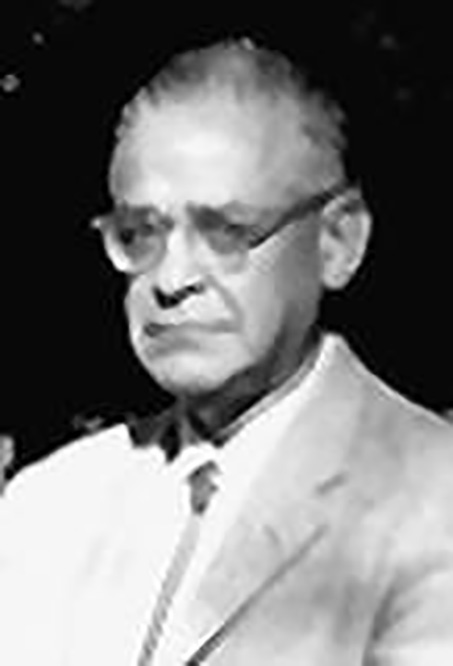
\includegraphics[width=.85\textwidth]{figures/bloch.jpg}
  \caption{Bernard Bloch}
  \label{fig:ch.structuralists.bloch}
\end{wrapfigure}
General practice in the period, following that of both {\Sapir} and
{\Bloomfield}, certainly did not provide for this ``desirable thing,''
but it was not until 1941 that the issue was made into a major point
of principle. \citet{bloch41:overlapping}, ``Phonemic Overlapping,''
distinguished two different senses in which the phonemic symbol
corresponding to a given sound might not be directly determined by its
phonetic character. One is relatively benign: it may be that the same
sound is assigned as a variant of two distinct phonemes, but in such a
way that its phonemic value is still uniquely determinate given the
phonetic context. This situation, called ``partial \isi{overlapping},'' is
exemplified by the \isi{flap} occurring medially in \ili{American English}
\emph{butter}. {\Bloch} suggests that a phonetically identical \isi{flap}
occurs for some speakers after [θ] in words like \emph{throw}. In the
former case the \isi{flap} is assigned to the /t/ \isi{phoneme}, while in the
latter it is assigned to /r/, ``but the intersection is only partial
and never leads to uncertainty or confusion: every such \isi{flap} between
vowels belongs to the [t] \isi{phoneme}, every \isi{flap} after a dental spirant
belongs to the [r] \isi{phoneme}'' \citep[279f.]{bloch41:overlapping}.

Much more pernicious, however, is the state of affairs characterized
by {\Bloch} as ``complete \isi{overlapping},'' where the same sound occurs as a
variant of more than one \isi{phoneme} in the same phonetic
environment. Several examples of this have arisen earlier in the
present book. The paradigm case is perhaps the assignment of final
voiceless obstruents in \ili{German}, \ili{Russian}, and other languages to voiced
phonemes in some forms but to voiceless ones in others; {\Bloch} cites
{\Bloomfield}'s analysis of reduced vowels in the same connection. He
argues that such analyses must be consistently excluded, for ``a
system in which successive occurrences of a given sound x under the
same conditions must be assigned to different phonemes necessarily
breaks down, because there can be nothing in the facts of
pronunciation—the only data relevant to phonemic analysis—to tell us
which kind of x we are dealing with in any particular utterance''
\citep[283]{bloch41:overlapping}.

{\Bloch}'s paper was enormously influential, and his position was quite
generally accepted by subsequent workers. The argument is that cases
of `complete \isi{overlapping}' must logically be excluded; but, as pointed
out by \citet[75]{kilbury76:morphophonemics}, the logic is less that
of demonstration than of definition. {\Bloch} defines phonemic analysis
in such a way that only ``the facts of pronunciation'' can be relevant
to it, and this does indeed entail the incoherence of analyses
involving complete \isi{overlapping}.

Given the climate of assumptions outlined in earlier sections above
(including an implicit theory of perception shared by most linguists,
and the denial of significance to any sort of `mental' constructs in
linguistic structure), the limitation proposed by {\Bloch} really did
seem to follow quite necessarily. This opinion could only be revised
in a rather different climate, in which there figured a notably richer
view of the process of perception, and in which language was once
again assumed to involve aspects of human cognitive organization and
not merely a network of directly corresponding stimuli and responses.

{\Bloch} showed plainly that the condition he had presented was more than
a slogan; it had serious consequences for the range of possible
analyses. He illustrates this with facts concerning \ili{American English}
vowels, which generally have longer variants when followed by voiced
sounds than by voiceless ones: for example, \emph{bid}, \emph{bed},
and \emph{bad} have phonetically longer vowels than \emph{bit},
\emph{bet}, and \emph{bat}. This also applies to the vowel [a]:
\emph{pod} has a longer vowel than \emph{pot}. Now in {\Bloch}'s dialect
there are a few words in which a long and a short [a] \isi{contrast}:
\emph{balm}, \emph{father}, and \emph{starry} for example have longer
vowels than those of \emph{bomb}, \emph{bother}, and \emph{sorry}. He
suggests that the long member of this pair also appears in the word
\emph{pa}. Now suppose that we wanted to treat the distribution of
\isi{vowel length} as non-phonemic (i.e., to assign both long and short
vowels to the same phonemes) where it is determined by a following
segment. In that case, however, we would confront the problem that
\emph{pa'd} (in \emph{pa'd go if he could}) is phonetically identical
with \emph{pod}; and thus the assignment of the vowel of \emph{pod} to
the `short-[a]' \isi{phoneme} while that of \emph{pa'd} is assigned to
`long-[a]' would result in complete \isi{overlapping}. This analysis must
thus be rejected.

\citet[284]{bloch41:overlapping} concludes from this that ``the neat
parallelism'' of the facts of \isi{vowel length} in vowels other than [a]
with those affecting [a] must thus be destroyed. In order to avoid
complete \isi{overlapping}, the relation between the vowels of \emph{pot}
and \emph{pod} must be treated as a relation between phonemes, while
that between \emph{bit} and \emph{bid}, for example, is a relation
between variants of the same \isi{phoneme}. He recognizes that this is an
unfortunate conclusion, but argues that it is the only scientifically
valid one. The explicit recognition of such unpalatable consequences
of the general principles of American structuralist \isi{phonemic theory} is
one of the most striking features of {\Bloch}'s work; indeed, it is
carried considerably further in his discussion of \ili{Japanese}
\citep{bloch50:japanese}.

There are alternatives to {\Bloch}'s analysis of \ili{English} \isi{vowel length}
which would have allowed him to preserve ``the neat parallelism''
among the vowels largely unimpaired, even on his assumptions. For
example, if the [a:] of \emph{pa}, though phonetically long, is
nonetheless taken as a variant (in final position) of the short /a/
\isi{phoneme}, the situation reduces to one of partial \isi{overlapping}. This is
beside the point, however. What is important is that, beginning with
this paper, American linguists thereafter accepted the exclusion of
complete \isi{overlapping} as a necessary condition on phonemic
analysis—regardless of the consequences for the coherence of the
resulting description. The necessity followed implicitly, as suggested
above, from more general assumptions about the nature of language. The
condition that \isi{phonemic representations} be uniquely recoverable from
phonetic data alone (together with its converse, that phonemic
\isi{representations} be uniquely translatable into phonetic form up to the
level of free \isi{variation}) was later given the name \isi{bi-uniqueness} by
\citet{harris44:yokuts}.

\largerpage
The essential motivation for the \isi{bi-uniqueness} requirement on the
relation between \isi{phonemic representations} and phonetic form was the
assumption that only ``the facts of pronunciation'' could possibly be
relevant to phonemic analysis. Another aspect of this same claim was
the explicit restriction that ``[t[here must be no circularity;
phonological analysis is assumed for grammatical analysis, and so must
not assume any part of the latter. The line of demarcation between the
two must be sharp.'' \citep[21]{hockett42:system}. `Grammatical'
(i.e., morphological or syntactic) analysis is based on a phonemic
representation; and if circularity is to be avoided in the resulting
description, facts from such `higher \isi{levels}' cannot play a role in
arriving at this representation. The point was sometimes presented in
this way, as a methodological one, and sometimes as a consequence of
\isi{bi-uniqueness} (following from the need to exclude non-phonetic factors);
but its substance was the general prohibition of analyses which `mixed
\isi{levels}'.

\begin{wrapfigure}[13]{r}{.35\textwidth}
  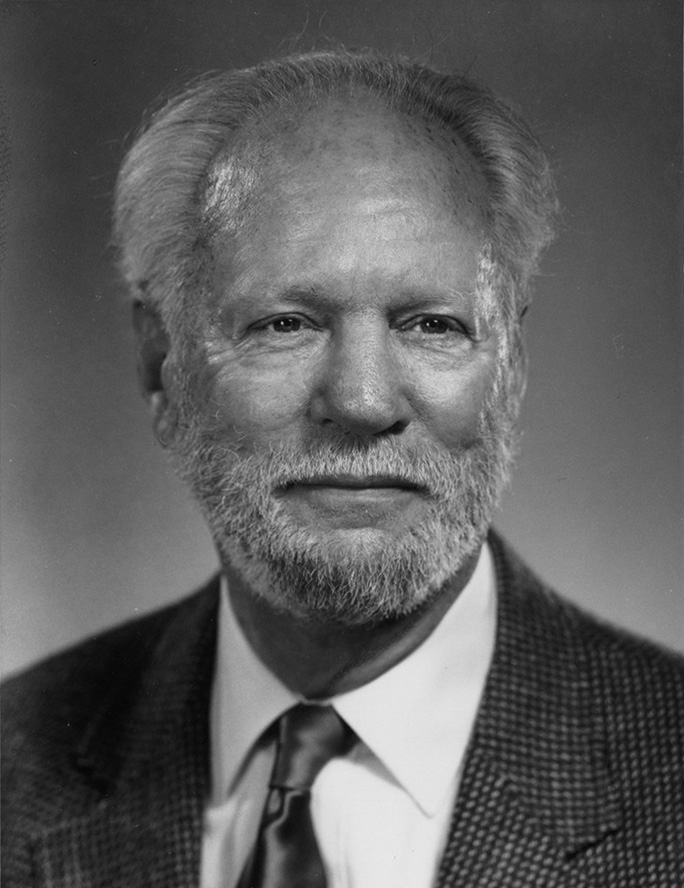
\includegraphics[width=.85\textwidth]{figures/Hockett.jpg}
  \caption{Charles Hockett}
  \label{fig:ch.structuralists.hockett}
\end{wrapfigure}
Of course, most analysts admitted the possibility that, after arriving
at a phonemic analysis, and then proceeding to analyze the morphology,
one might go back and revise the initial phonemic system in light of
the morphology so as to make the latter more coherent. After all, it
was known \citep{chao34:non-uniqueness} that phonetic data typically
support more than one possible valid phonemicization, and there was no
reason not to choose that analysis which yielded the most satisfactory
system at all \isi{levels}. It was argued explicitly (e.g., by
\citealt{hockett47:problems}) that such a procedure was
defensible—provided that the phonemic system chosen was one that,
considered apart, satisfied the condition of biuniqueness and did not
involve essential reference to other \isi{levels} of analysis. `Mixing
\isi{levels}' was a perfectly satisfactory expedient as a field procedure,
as long as it left no traces in the resultant grammar. This
possibility follows from (and also illustrates) the separateness of
actual field procedures and the abstract, idealized procedures that
constituted the definition of constructs such as `phonemic
representation' within the linguistic theory of American
\isi{structuralism}.


\largerpage
Some linguists rejected the prohibition against \isi{mixing levels},
however. The best-known arguments against this requirement were those
of \citet{pike47:gppa,pike52:mogp}, under the heading of ``grammatical
prerequisites to phonemic analysis.'' {\Pike} argued that a satisfactory
phonemic analysis might require access to information about the
grammatical structure of forms, and he provided a number of cases in
which such information seemed clearly relevant.

\begin{wrapfigure}{l}{.45\textwidth}
  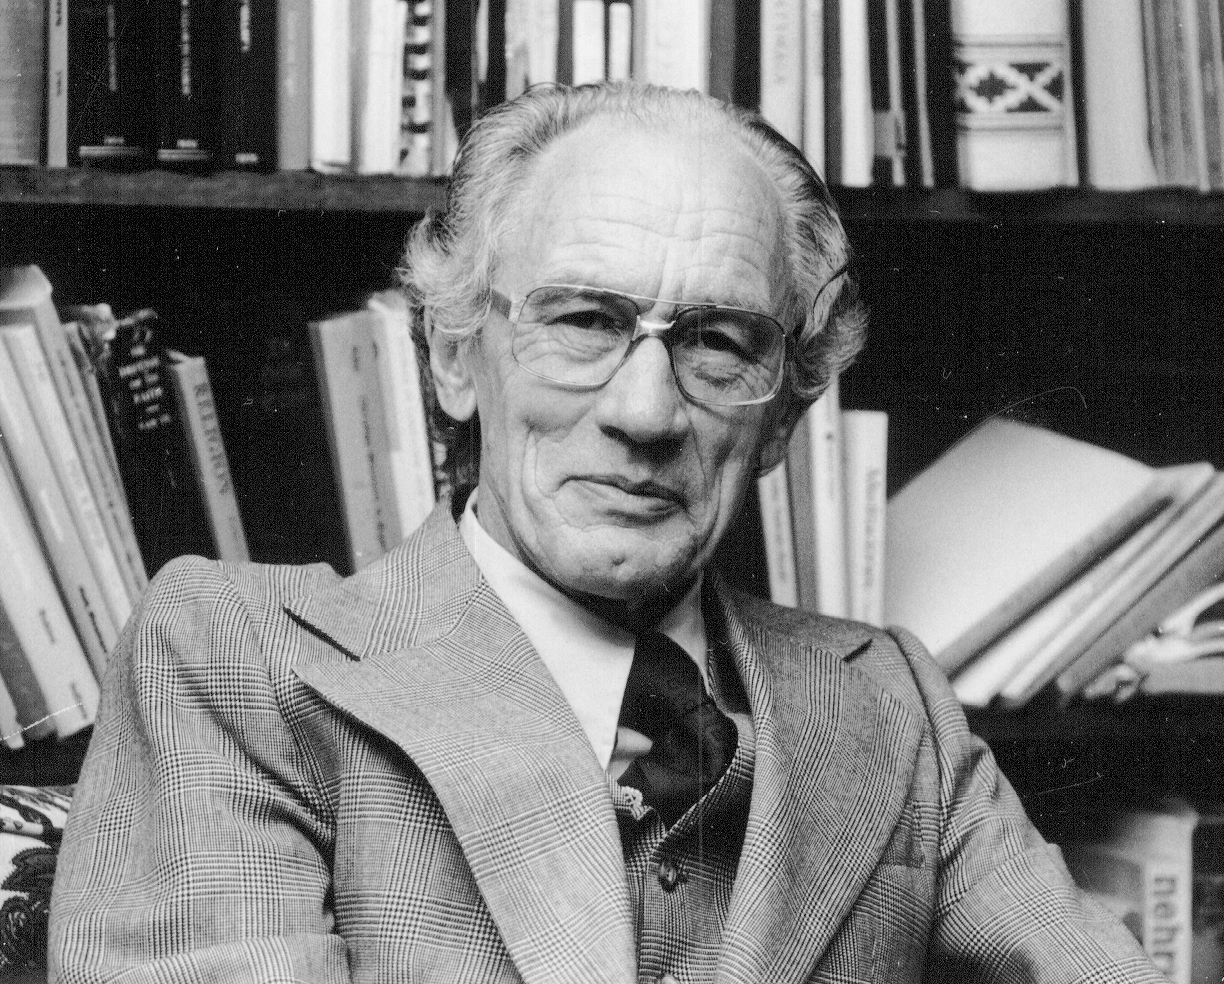
\includegraphics[width=.85\textwidth]{figures/Kenneth_L._Pike.jpg}
  \caption{Kenneth L. Pike}
  \label{fig:ch.structuralists.pike}
\end{wrapfigure}
Pike\ia{Pike, Kenneth L.}'s examples all fall into the same class with one presented
earlier by {\Bloomfield} in his analysis of [x]/[ç] in \ili{German}: all
involve the role of grammatical \isi{boundaries} in conditioning the
appearance of particular variants of phonemic units. The indication of
\isi{boundaries} of course constitutes a rather limited use of grammatical
information: much less radical, for example, than would become common
in early generative work, where it was assumed that \isi{phonological rules}
could have access to a complete, structured phrase marker with
hierarchical information, identification of morphological categories,
etc.

Pike\ia{Pike, Kenneth L.}'s arguments were not in general accepted by the mainstream of
American structuralist phonemicists, since the admission of inaudible
grammatical factors in a phonemic description would have dealt too
severe a blow to the conception of `phonemic representation' they
assumed. An alternative was quickly found, however, which allowed for
most of {\Pike}'s cases while maintaining at least the semblance of
independence from `grammatical prerequisites'. This was the positing
of additional phonemic elements, called `\isi{junctures}', whose realization
generally consisted not in some actual segmental element, but rather
in their distinctive conditioning effect on other phonemes.

\citet{moulton47:juncture}, for example, posits an element /+/ of
``open juncture'' (a notion going back to
\posscitet{trager.bloch41:syllabics} earlier suggestions) in his
analysis of \ili{German}. ``This \isi{phoneme} has two allophones: at the
beginning or end of an utterance it appears as a pause of indefinite
duration; within an utterance it appears as a brief pause or, in free
\isi{variation}, as zero'' \citep[223]{moulton47:juncture}. The extent to
which internal instances of /+/ in \ili{German} (such as those posited
before the diminutive element -\emph{chen}) actually can be realized
by an overt pause is unclear, but this is not of course their main
function. What is important is the fact that ``we may assume this
element wherever we find a pause (of whatever duration) and, in
addition, wherever we find (1) aspirated /p t k/; (2) a glottal stop;
and (3) the sound [ç] following (phonetically) a central or back vowel
or semivowel''.

Moulton\ia{Moulton, William} is thus able to achieve {\Bloomfield}'s reduction of [x] and [ç]
to a single \isi{phoneme}, but without referring directly to grammatical
structure, by referring instead to a phonemic element which is defined
in (superficially) phonetic terms as potential pause alternating with
zero. Of course, he observes somewhat disingenuously, ``the places
where /+/ occurs usually coincide with syntactic and morphological
\isi{boundaries}'' \citep[224]{moulton47:juncture}; but this is not a
problem, since the definition of the element does not refer to such
\isi{boundaries}. For further support of the independence of /+/ from
grammatical structure, he cites a few borrowings with exceptional
\isi{stress} in which internal instances of /+/ might be posited for reasons
unrelated to \isi{boundaries}.

Ingenious uses of `juncture phonemes' allowed descriptions to maintain
the letter of the prohibition against the appearance of grammatical
information in phonemic analyses, while evading some of the worst
consequences of a restriction to ``the facts of pronunciation.'' The
consequence, however, was a considerable enrichment of the notion of
`\isi{phoneme}': when the phonetic manifestation of a `\isi{phoneme}' of `close
juncture' (aside from its effect on adjacent phonemes) could be
defined precisely as an absence of potential pause, it is clear that
analyses had come a long way from the notion of phonemes as discrete,
additive signaling units. Further enrichment of the phonemic \isi{concept}
came with the attempt (especially in the mid- to late 1950s) to
accommodate the facts of \isi{stress}, distinctive \isi{pitch}, and
intonation—together with junctural phenomena—into a unitary inventory
of phonemic units homogeneous in their linguistic status with
segmental phonemes. Since the \isi{phoneme} was taken as the `atomic'
building block of \isi{contrast}, however, there was little alternative,
whenever new dimensions of \isi{contrast} were noticed, to incorporating
these facts into an ever-widening conception of the \isi{phoneme}.

The concentration of attention in \isi{American structuralism} on the nature
of the \isi{phoneme} continued to characterize theoretical discussion
throughout the 1950s, leaving the status of rule-governed relations
between phonemes in a somewhat ambiguous position. On the one hand,
analysts considered such \isi{regularities} (especially those expressing
distributional facts) important enough to warrant a place in
descriptions and to influence (if not completely determine) phonemic
analyses in the name of `\isi{pattern congruity}'. On the other hand, since
a phonological description was conceived first and foremost as a
theory of \isi{phonemic representations} in a particular language, the only
way such considerations could enter the picture was as part of the
definition of individual phonemes.

Recall that the theory itself was presented in the form of a set of
analytic procedures, which if followed were supposed to lead to
objects of the intended sort. This entailed that phonological `rules'
only had status insofar as they could be incorporated in
procedures. As opposed to the (static) \isi{representations} that are
arrived at by applying them, no particular `reality' was attributed to
the procedures themselves; and thus it was not really possible to
sustain rational arguments about the form of possible rule-governed
\isi{regularities} that might occur in natural languages. In the absence of
any sort of independent criterion that might decide which \isi{regularities}
were linguistically relevant and which accidental (or simply
non-linguistic), discussion tended to be quite anecdotal and
aprioristic.

The concentration of phonological attention on questions of the nature
of \isi{representations}, with the consequent marginality assigned to
rule-governed \isi{regularities} in linguistic structure, has by no means
been confined to American structuralists among theorists of natural
language. However, some of the characteristic features of this theory
reinforced this tendency here more than in other theories. Among these
are the rigorous attention to the `separation of \isi{levels}', and the
concomitant exclusion of most alternations from phonological
relevance, together with the general requirement that phonemic
\isi{representations} be bi-uniquely related to phonetic data, which excludes
even phonologically conditioned alternations between phonemes from
relevance. Neither situation was considered wholly satisfactory by the
linguists involved, but on the basis of their overall principles no
alternative seemed to present itself. Excluded from a central position
in the theory, \isi{regularities} other than simple matters of distribution
were either relegated to the non-systematic status of `pattern
congruity', or else treated in twilight zone of \isi{morphophonemics}. It is
to this aspect of American structuralist theory that we turn next.

\section{American structuralist morphophonemics}
\label{sec:struct-morphophonemics}

The history of morphophonemic description within \isi{American
structuralism} is a somewhat uneasy one. Facts regarding all but the
most superficial alternations between related forms are intrinsically
beyond the scope of such a theory of phonology, since `relatedness'
between forms is not deducible from ``the facts of pronunciation
alone.'' Any sort of description that attempts to reduce related
elements to an underlying unity, so long as the elements themselves
involve distinct phonemes (in the bi-unique sense of American
\isi{structuralism}), must therefore necessarily lie outside of phonology.

As a result, American structuralists had recognized more or less from
the beginning a discipline of `morpho(pho)nology' or
`\isi{morphophonemics}'. According to \citet{swadesh34:phoneme}, this part
of linguistics dealt with two things: ``the study of the phonemic
structure of morphemes,''\footnote{The present writer's reservations
  about the utility of the notion of `morpheme' as developed in
  structuralist theories \citep{sra12:the-morpheme} will be set aside
  for the purposes of this discussion.} and also ``the study of
interchange between phonemes as a morphological process.'' Definitions
of the scope of \isi{morphophonemics} offered by subsequent writers
(including {\Bloch}, {\Harris}, {\Hockett}, {\Wells}, and others) varied somewhat
as to whether both of these were to be handled in the same part of the
grammar. Everyone was agreed that ``interchange between phonemes,'' or
the study of \isi{systematic relations} in shape of related forms, was a
part of \isi{morphophonemics} (assuming there was such a field); the
differences hung on whether the statement of \isi{regularities} of morpheme
shape (what would later be called `morpheme-structure rules' within
\isi{generative grammar}) belonged there too. The issue seems largely
terminological, however, since no one ever claimed that anything much
depended on the decision. Our interest here is primarily in the
treatment of \isi{regularities} in the shapes of related (rather than
individual) forms, and we will use the term `\isi{morphophonemics}' in that
sense.

The earliest American phonemic work assimilated many facts of
\isi{morpho\-phonemic alternation} to the rest of the phonology. This was
certainly true for {\Sapir}, and to a limited extent (as
discussed above) for {\Bloomfield} as well. At least by 1939, though,
{\Bloomfield} also distinguished a separate treatment of \isi{morphophonemics}
(in the specific, restricted sense of internal sandhi alternations)
from phonemics. As discussed in chapter~\ref{ch.bloomfield},
{\Bloomfield}'s technique for morphophonemic description was derived from
Pāṇini: it consisted in the setting up of `base forms', to which a set
of ordered rules applied one at a time to derive eventually the
surface (phonemic) form. We can say, in fact, that while {\Bloomfield}
held a `partially specified surface variant' view of phonemic
structure, he took a `basic variant' view of morphophonemic
structure—extending the terminology of chapter~\ref{ch.saussure_sound}
to this new domain.

A combination of phonological and morphophonemic facts also appears in
\posscitet{trager34:russian} paper on \ili{Russian}, as noted
above. Interestingly, this paper stimulated {\Trubetzkoy} to write to
{\Jakobson} that although {\Trager}'s analysis of \ili{Russian} was completely off
the mark, his descriptive framework and terminology seemed to be an
attempt to imitate morphophonemic work of the Prague school
phonologists. \posscitet{swadesh34:phoneme} paper, which explicitly
distinguishes phonology from \isi{morphophonology} in much the same way
{\Trubetzkoy} did, also seemed part of an American attempt to imitate the
Praguians. In retrospect, although there is some clear borrowing of
Praguian terminology, the notion that {\Trager} and {\Swadesh} were trying
to be like {\Trubetzkoy} and {\Jakobson} seems somewhat far-fetched. The
distinctions between phonology and \isi{morphophonemics} were still blurred,
just as they had been in the work of {\DeCourtenay}—and
American phonologists, like those in Prague, were attempting to draw
lines in accord with their understanding of the nature of phonemic
structure.

As `pure' phonemic doctrine developed, it came to exclude the
treatment of morphophonemic alternations more and more definitively
(both in America and in Europe). This did not, of course, prevent
linguists from recognizing that there were indeed systematic
relationships of this sort whose description belonged in a
comprehensive account of language structures. But since these
relationships could not be accommodated within the phonology
\emph{sensu stricto}, the only place for them was in the description
of morphology. As a result, the subsequent history of \isi{morphophonemics}
(at least in America) is entangled with the emergence of a distinctive
view of the nature of morphemes.

{\Bloomfield}'s approach to morphophonemic description in terms of basic
variants and ordered rules came in for a certain amount of criticism
from the `post-Bloomfieldian' generation. To them, despite
{\Bloomfield}'s specific disclaimers, such a description looked
suspiciously like a historical account. What, after all, could such a
sequential application correspond to except the sequence of historical
changes that had given rise to a present-day \isi{alternation}? Linguists
such as {\Wells}, Lounsbury\ia{Lounsbury, Floyd Glen}, and others in their methodological
discussions of \isi{morphophonemics} felt that it was necessary to maintain
a strict exclusion of anything of the sort from synchronic grammars,
and thus rejected {\Bloomfield}'s descriptive technique. In general, this
formed part of a more general tendency in American linguistics to
eliminate dynamic, process-like statements deriving forms from one
another or from more basic forms, in favor of static descriptive
accounts which directly characterized the range of occurring
forms. This preference results, of course, from the underlying
assumption that it is only the \isi{representations} of individual forms
that linguistics should focus on, since only the forms themselves are
observable and thus `real'.

\begin{wrapfigure}{r}{.35\textwidth}
  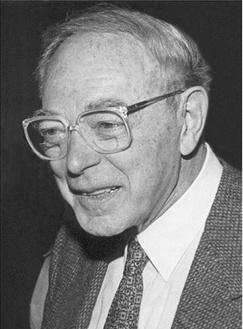
\includegraphics[width=.85\textwidth]{figures/Zellig_Harris.jpg}
  \caption{Zellig Harris}
  \label{fig:ch.structuralists.harris}
\end{wrapfigure}
The alternative to process-type descriptions which developed centered
around the method of `\isi{morpheme alternants}'. This was first discussed
in detail by \citet{harris42:alternants}, and arises as an answer to a
problem concerning the nature of the morpheme. Following {\Bloomfield},
{\Harris} starts from the definition that ``every sequence of phonemes
which has \isi{meaning}, and which is not composed of smaller sequences
having \isi{meaning}, is a morpheme''
\citep[169]{harris42:alternants}. Morphemes are thus identified with
particular sequences of phonemes; but this has the unfortunate result
of ``dissociat[ing] certain morphemes which we wish, because of the
grammatical structure, to unite''. In the simplest case, the three
forms /-əz/, /-z/, and /-s/ of the \ili{English} \isi{regular} plural ending
constitute three different \isi{phoneme} sequences, and thus three different
morphemes on this definition. From the point of view of the syntax, we
obviously want to treat these as the same morpheme; which means we
must revise our notion of `morpheme'.

{\Harris}'s procedure is first to isolate the minimal meaningful
sequences of phonemes, as before, but to call them ``morpheme
alternants'' instead of morphemes. He then groups together as a single
``morpheme unit'' any set of \isi{morpheme alternants} that have the same
\isi{meaning} and which are in \isi{complementary distribution}. The model is
obviously the same as the phonological one: a morpheme on this view
({\Harris}'s ``morpheme unit'') is a set, which is related to its members
or allomorphs (a term introduced by {\Nida} to replace {\Harris}'s
``morpheme alternant'') just as a \isi{phoneme} is a set consisting of its
allophones.

Having organized \isi{morpheme alternants} into morphemic units, we can now
examine the differences among the alternants of individual morphemic
units. ``If we find another morpheme unit having an identical
difference between its alternants, we can describe both units
together. Thus between \emph{knife} and \emph{knive}-, which make up
one unit, the difference is identical with the difference between
\emph{wife} and \emph{wive}-, which make up another, and with the
difference between \emph{leaf} and \emph{leave}-, and so on. Instead
of listing both members of each unit, we now list only one
representative of each unit with a general statement of the difference
which applies to all of them: Each of the units \emph{knife},
\emph{wife},\ldots, has an alternant with /v/ instead of /f/ before
/z/ `plural' '' \citep[172f.]{harris42:alternants}.

This method of description is not dramatically different at first
sight from an analysis with base forms and rules to convert them into
surface forms, but there are important distinctions nonetheless. Note
that {\Harris} does not actually \emph{derive} the form \emph{knive}-
from \emph{knife} by a rule turning /f/ into /v/: rather the
representation \emph{knife}, together with the fact that this morpheme
appears on the relevant list, serves as an abbreviation for the two
alternants \emph{knife} and \emph{knive}-, with one alternant
appearing in a particular environment and the other appearing
elsewhere. As far as the language is concerned, the morpheme simply
has two alternants, with the same status: one is not derived with
respect to the other.

Another example of the same sort is provided by
\posscitet{harris45:rvw.emeneau} review of \posscitet{emeneau44:kota}
analysis of the Dravidian language Kota. {\Emeneau} (a student of
{\Sapir}'s) describes the patterns of \isi{alternation} in that language by
establishing a \isi{base form} for every morpheme in the language. These
base forms are composed not of phonemes, but of morphophonemes, each
of which can be realized by one or more phonemes, depending on the
environment in which they occur. Words are constructed by
concatenating the necessary set of morphemes, and the sequence of
morphophonemes obtained in this way is then converted by a set of rules
that replace the individual morphophonemes appropriately. Another set
of rules of external sandhi takes the \isi{representations} thereby obtained
of words in sequence in a larger construction, and converts these to a
phonemic form. In his discussion, {\Harris} first observes that the two
sets of rules (which are often the same, can be reduced to one by
recognizing boundary elements (such as that between words) in the
statement of the environments for conversion of morphophonemes into
phonemes. He then suggests, however, that a preferable account would
simply list for each morpheme the complete set of phonemic
realizations which correspond to it, providing each such morpheme
alternant with a statement of its conditioning environment---entirely
parallel to his account of the the \emph{knife}/\emph{knive}-
\isi{alternation}.

Alternants are grouped together into morpheme units in the same way
regardless of whether the differences among them are systematic or
not: \emph{am}, \emph{are}, \emph{is}, etc. are grouped together in
the same way as the alternants of the \isi{regular} plural or
\emph{knife}/\emph{knive}-. Where the \isi{variation} is recurrent, we can
state it in a descriptive formula, and then summarize the allomorphs
of a given morpheme by a representation which is not in itself a
morpheme alternant, but which in conjunction with the formula allows
us to determine the actual \isi{morpheme alternants}.

Later in the paper, {\Harris} makes clearer the static, formulaic
character of the \isi{representations} which are provided for individual
morpheme units. He also introduces a minor revision. Instead of
writing /nayf/ for `knife', and then including this element on a list
of those to which the descriptive statement of the \emph{f}/\emph{v}
\isi{alternation} applies, we can write such elements with a special
morphophonemic symbol /F/: thus, /nayF/ is subject to the \isi{alternation},
but /fayf/ is not.

It is important to be clear about the status of the elements such as
this /F/. They are clearly not intended to be additional phonemes of
the system, or to have a direct phonetic interpretation at
all. Rather, /F/ is an abbreviation for the formula: (phonemic) /v/
before the plural /-z/, (phonemic) /f/ elsewhere. This is quite
parallel to the conception of the \isi{phoneme} as a set of allophones, each
with a condition on its appearance: the differences are a) that the
members of the set desiganted by a morphophoneme are themselves
phonemes, rather than phonetic segments; and b) that the conditions
associated with the members of the set include information (such as
the presence of {[+Plural]}) that is not purely phonological.

In this way, morphemes are provided with unitary \isi{representations}
insofar as their alternants are systematically related, but the role
of these \isi{representations} is to abbreviate the list of occurring
phonemic alternants, and nothing more. Morphemes are units; they are
sets, composed of alternants which are also (as phonemic sequences)
units. A unitary representation is simply a convenient abbreviation
for the set of alternants united in a given morpheme, employed where
possible, but having no other systematic status.

Morphophonemic symbols such as /F/, which serve as abbreviations for a
set of alternating phonemes under various conditions, are parallel to
the morpho(pho)nemes posited by {\Trubetzkoy} (chapter~\ref{ch.prague}). In
both cases, the only condition on the formation of a morphophoneme is
that the conditions of occurrence of the various alternating phonemes
subsumed under it be statable and recurrent. No requirement at all is
imposed that the \isi{alternation} be phonetically coherent or `natural':
the morphophonemic symbol simply replaces a list of individual
phonemes, each of which has some particular environment in which it
occurs.

We can \isi{contrast} this sort of abstract morphophonemic symbol with
another usage, which is found in {\Bloomfield}'s work. In his description
of \ili{Menomini}, {\Bloomfield} represents morphological elements as abstract
base forms, which are composed for the most part of phonemic
elements. Their interpretation is such that, if no rule applies to
change a given \isi{phoneme} into some other, it is realized as
such. Certain symbols, however, do not have a direct phonemic
interpretation but are abstract: these must be replaced by some
phonemic symbol (or, of course, deleted) if the resultant
representation is to be well formed. Such abstract symbols are
typified by the element /N/ used (in \citealt{bloomfield62:menomini})
to represent an /n/ which fails to undergo \isi{palatalization}: after the
\isi{palatalization} rule applies, changing /n/ to /s/ in certain
environments, all instances of /N/ are replaced by /n/, thus merging
with remaining instances of this \isi{phoneme}.

In every case, {\Bloomfield} uses abstract (i.e., nonphonemic) symbols in
base forms to represent the fact that certain elements which are
otherwise phonemically unitary show two distinct types of behavior
with respect to particular rules. Thus, /n/ and /N/ are both realized
as phonemic /n/, and differ only in that /n/ is subject to a
\isi{palatalization} which /N/ does not undergo. We can distinguish this
sort of abstract symbol from that represented by {\Harris}'s /F/, in that
{\Bloomfield}'s /N/ (and other such symbols in his grammar) is simply
used to indicate an /n/ which behaves unusually. In generative terms,
the difference between /N/ and /n/ is that one bears an exception
feature which the other does not. {\Harris}'s /F/, on the other hand,
represents a collection of elements which are in principle completely
arbitrary (even though phonetically similar in this case), phonemes
related only in that they occur in corresponding places in related
allomorphs of the same morphemes under the conditions of an
\isi{alternation}.

Naturally, it is possible to express the `Bloomfieldian' sort of
morphophoneme in terms of the other type. We can say that \ili{Menomini}
/N/ is represented by simple phonemic /n/ in all environments, while
/n/ is a morphophoneme represented by phonemic /s/ in some
environments, and by phonemic /n/ in others. Interestingly,
\citet{bloomfield:menomini_morphophonemics} uses the special symbol
/N/ for the alternating segment, and /n/ for the non-alternating. This
usage is more nearly in line with that of other writers on
\isi{morphophonemics}, and with the conception of morphophonemes as formulas
for alternations; perhaps the reversal of usage between
\citealt{bloomfield:menomini_morphophonemics} and
\citealt{bloomfield62:menomini} reflects a difference in conception.

One of the most important early American structuralist papers on
\isi{morphophonemics}, that of \citet{swadesh.voegelin39:alternation},
illustrates both of these usages for morphophonemic symbols
simultaneously. On the one hand, in discussing the role of abstract
morphophonemic symbols in descriptions, {\Swadesh} and {\Voegelin} treat the
same \ili{English} example (\emph{wife}/\emph{wives},
\emph{leaf}/\emph{leaves}, etc.) that {\Harris} would discuss a few years
later, and propose the same account: a morphophoneme /F/, which serves
as an abbreviation for the \isi{alternation} `\isi{phoneme} /v/ before plural /z/,
\isi{phoneme} /f/ elsewhere'. On the other hand, in their discussion of
\ili{Tübatulabal}, they use morphophonemes in the way {\Bloomfield} had: that
is, to represent two variants of the same surface \isi{phoneme} which differ
in their behavior with respect to particular rules of the grammar.

\ili{Tübatulabal} exhibits an extensive network of alternations between long
and short vowels. {\Swadesh} and {\Voegelin} show that in a number of cases,
vowels that would otherwise be long appear short when followed by a
voiceless obstruent, while either a long or a short vowel may be
followed by a voiced obstruent. This suggests a rule shortening vowels
before voiceless (but not voiced) obstruents. Unlike the obstruents,
the nasals, semivowels, liquid /l/, and \isi{laryngeals} (/h/ and /ʔ/) do
not show a distinction between phonetically voiced and voiceless
forms. In some instances, however, vowels are shortened before members
of this class, while in others they are not. Among the non-obstruents,
then, we have two sorts of morphophonemic behavior: some segments
trigger shortening, while others do not, although there is no phonetic
(or, \emph{a fortiori}, phonemic) difference between the two.

An obvious morphophonemic solution would be to set up two classes of
non-obstruents—underlyingly voiced versus voiceless—in parallel with
the two (phonetically motivated) classes of obstruents. It could then
be stated that vowels are shortened before voiceless seg\-ments but not
before voiced; and, subsequently, voiced and voiceless non-obstruents
are merged (as phonetically voiced seg\-ments in the case of the nasals,
and /l/, and as voiceless for the \isi{laryngeals}). Interestingly, {\Swadesh}
and {\Voegelin} do not propose this solution. They do indeed set up two
classes of non-obstruents, but instead of treating the difference as a
matter of \isi{voicing}, they simply call one class ``shortening
\isi{consonants}'', and the other class ``neutral'' or ``non-shortening''. A
phonetic interpretation is almost ostentatiously avoided.

A similar analysis is provided for the vowels. Some vowels in
\ili{Tübatulabal} show up as long unless affected by a shortening rule;
while others show up short unless affected by a (positional)
lengthening rule. Again, the obvious analysis would seem to be to
distinguish the two classes phonetically, as underlying long versus
short vowels. Instead, {\Swadesh} and {\Voegelin} distinguish `heavy' from
`light' vowels, and use a different diacritic to mark `heavy' vowels
in morphophonemic \isi{representations} from that used to mark long vowels
in phonemic forms. Both in this case and in that of the \isi{consonants},
the interpretation is clear: differences between morphophonemic
symbols do not correspond directly to phonetic or phonemic differences
but to differences between two sorts of behavior that may be shown by
the `same' surface phonemic segment type—exactly as in {\Bloomfield}'s
usage. This variety of abstract morphophonemic symbol can be
distinguished from that of the /F/ in \emph{leaf}/\emph{leaves}, but
both sorts of morphophoneme are quite distinct from phonetic or
phonemic elements.

\section{Rule interactions and the nature of descriptions}
\label{sec.struct.interaction}
\largerpage
In addition to the status of elements in morphophonemic
\isi{representations}, other issues of importance which can be identified in
the morphophonemic theories of American structuralist writers include
their treatment of rule interaction or ordering. Recall that, in
{\Bloomfield}'s method of description, the rules of a morphophonemic
analysis are applied in a sequence (or ``descriptive order''), with
each rule applying to the result of applying the previous
rule. The precise order of application of the rules of a grammar is a
matter to be specified in the grammar itself. To say that one rule
`precedes' another in a description means more precisely that the
results of the first rule's application are presupposed by the second,
and, furthermore, that any information destroyed by the first rule is
not accessible to the second \citep[see][]{sra03:iel2.ordering}. For
{\Bloomfield}, as for generative phonologists (at least until about
1970),  relations of presupposition among rules were to be
specified in the grammars of individual languages just like any other
aspect of the rules themselves. Other writers on \isi{morphophonemics},
however, while they assume something like a relevant applicational
sequence for the rules of the grammar, make assumptions that are
rather different from {\Bloomfield}'s.

It would take us too far afield here to examine in detail the
alternatives to a specified descriptive order which can be found in
American structuralist morphophonemic descriptions \citep[for
extensive discussion, see][]{kenstowicz75:application}, but one
important tradition can be noted, which Kenstowicz\ia{Kenstowicz, Michael} traces to the work
of {\Sapir}. I noted in chapter~\ref{ch.sapir} that {\Sapir} assumed that
rules applied in a sequence, but a sequence which was predictable from
general principles rather than specified in the grammar. In addition,
{\Sapir} allowed rules to refer to the difference between `organic'
elements (those present in underlying forms), and `inorganic' ones
(those produced by the operation of a rule).  The reference to
`organic' vs. `inorganic' elements is a distinction available to any
rule of the grammar, and allows rules to have access to information
which previous rules have destroyed. This possibility arises in the
case of an `organic' segment which has been altered by a rule, but
whose underlying source is still accessible to subsequent rules.

References of this sort to the underlying value of a segment which has
in fact been altered by a rule are found in a number of papers in the
1930s, 1940s, and 1950s, (including
\citealt{swadesh.voegelin39:alternation}, in particular) as documented
by \citet{kenstowicz75:application}. In general, the assumptions
underlying rule interactions within particular grammars went
un-discussed in the theoretical literature of the time, and it is not
always clear how much significance to attribute to the assumptions
which can be shown \emph{ex post facto} to be necessary in order to
get a particular description to yield the correct results. In at least
one case, however, the particular issue of reference to basic versus
derived forms is specifically addressed.

\citet{harris:methods}, dealing with the nature of morphophonemic
description, raises the question of the role of descriptive order. He
cites rules of {\Bloomfield}'s from \ili{Menomini}, where (a) morpheme-final
/n/ is replaced by /s/ before /e/ or /y/; and (b) final vowels are
dropped. ``When we now meet /ōs/ `canoe', /ōnan/ `canoes', we
recognize that this \isi{alternation} can be stated as the sum of the
previous two. However, this can only be done if we set up a
morphophonemic /ōn-e/ and then apply our two alternations in the order
in which they are stated above; if we first drop the /e/, we will have
lost the condition for then replacing the /n/ by /s/''
\citep[237]{harris:methods}.

\begin{wrapfigure}{r}{.4\textwidth}
  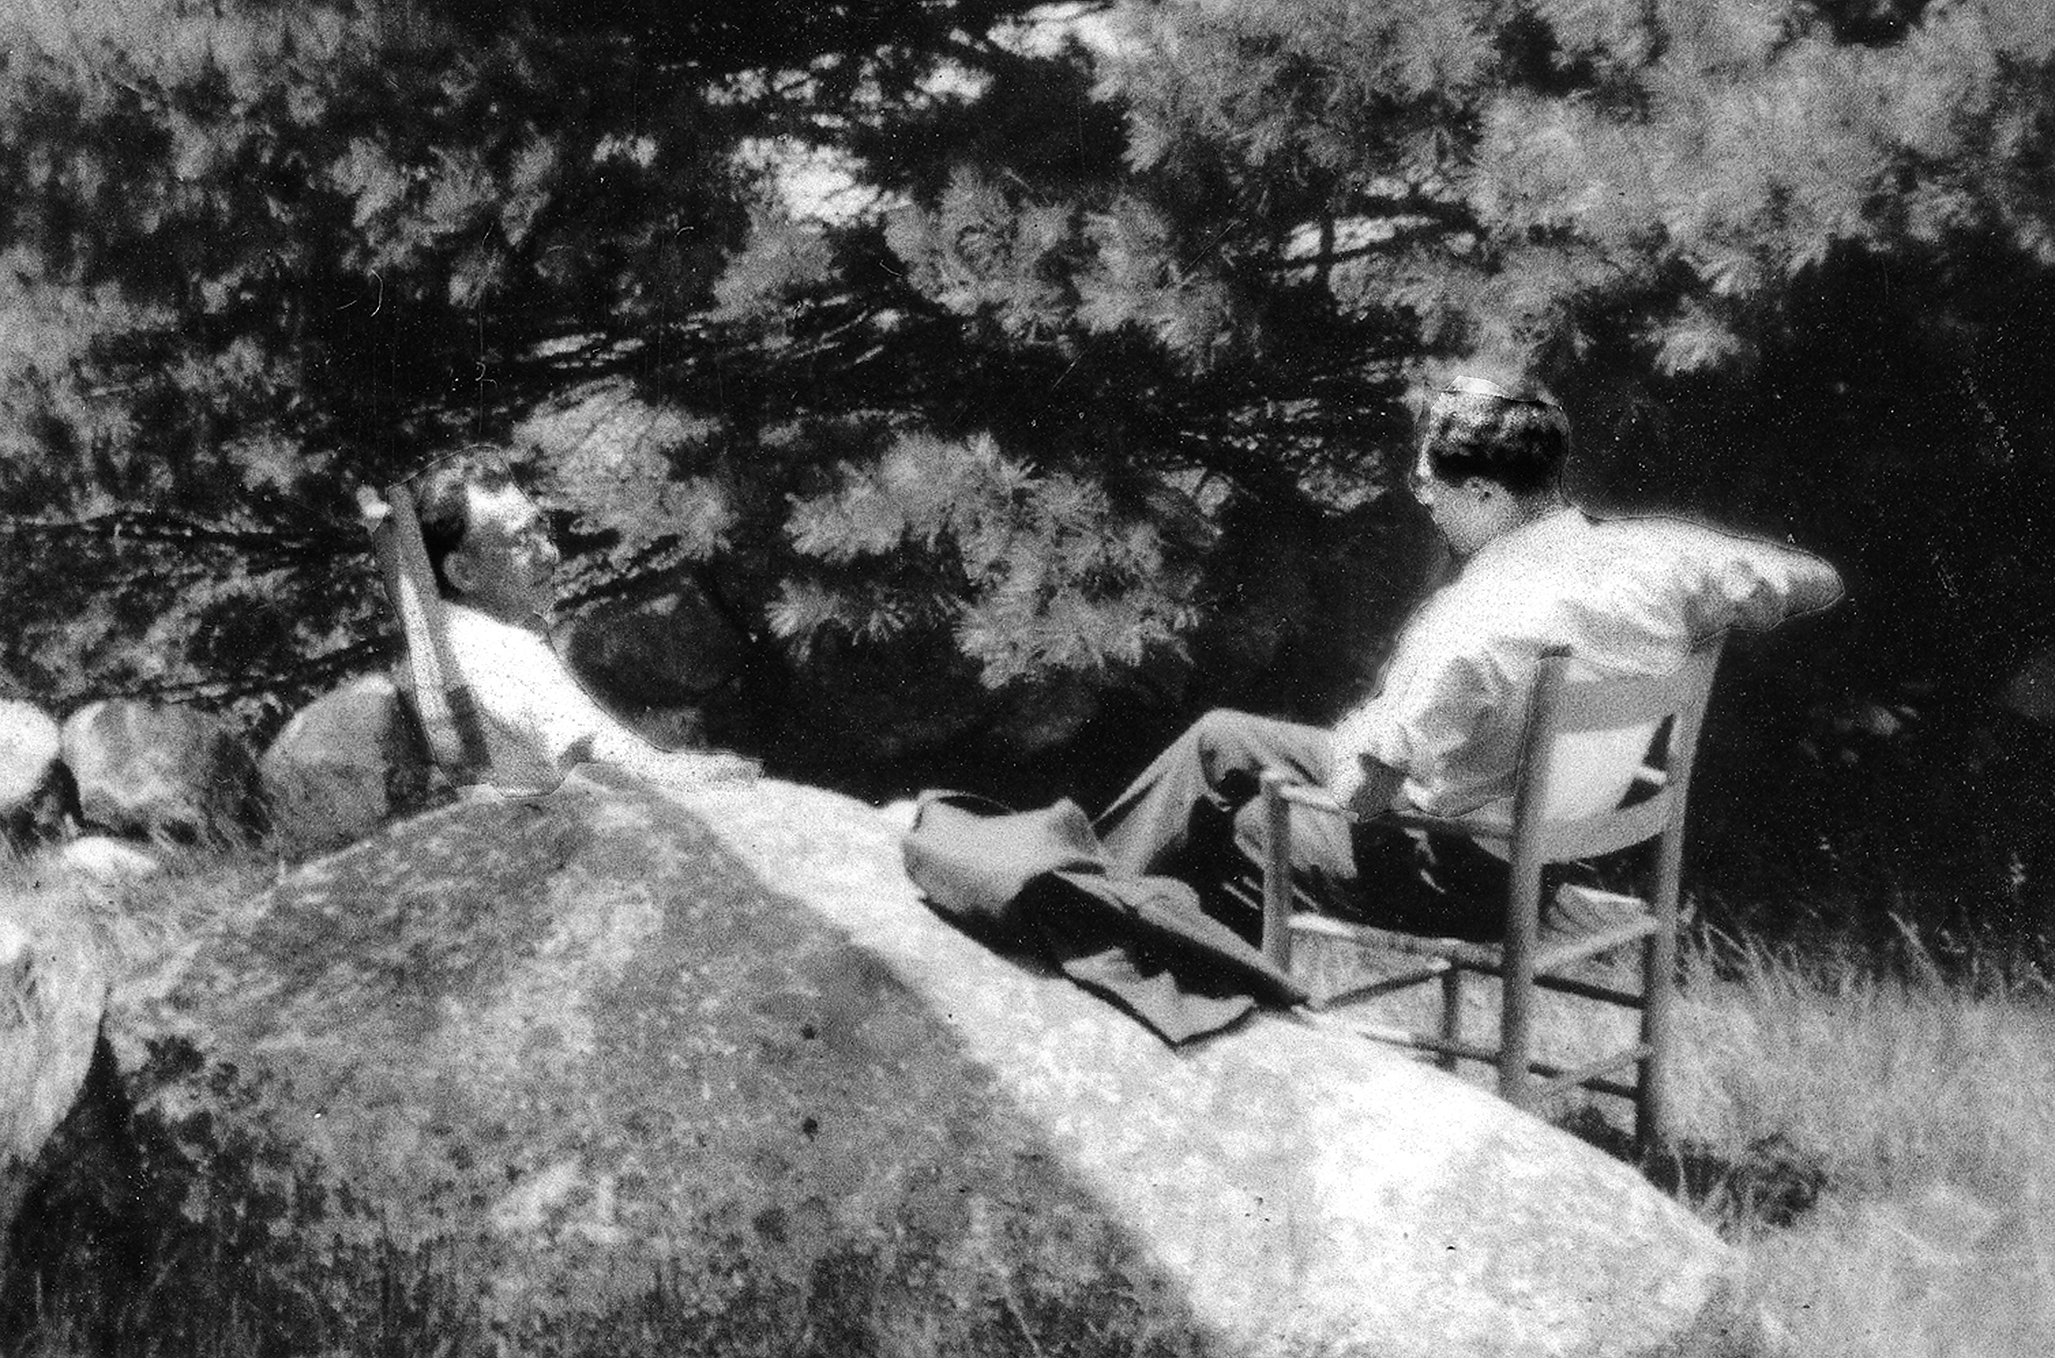
\includegraphics[width=.95\textwidth]{figures/Sapir-Harris.jpg}
  \caption{Edward Sapir (left) and Zellig Harris (New Haven, ca. 1937)}
  \label{fig:ch.structuralists.sapir_harris}
\end{wrapfigure}
Harris\ia{Harris, Zellig} here appears to commit a logical error which is in fact rather
common in the subsequent literature (including some generative
discussions). He seems to argue that this example demonstrates a need
for descriptive order, when in fact it simply shows that if the rules
involved are applied in an order, it makes a difference which
order. \citep[For some discussion of such cases,
see][ch. 5.]{sra74:orgphon} True, applying the rules in the reverse of
the order presented above yields an incorrect form (/ōn/); but it is
also true that if both rules apply to the same representation (the
underlying form) independently of one another (i.e., if the rules
apply simultaneously), the correct result is also obtained. What is
necessary is simply to ensure that when the rule replacing /n/ by /s/
applies, the presence of a final /e/ is still accessible. This can be
achieved either by (a) having the rule dropping final vowels apply
only after the rule of /n/ to /s/; or (b) allowing the /n/ to /s/ rule
to examine the \isi{underlying representation}, regardless of whether final
vowel loss also eliminates the /e/ from the surface form.

Despite the apparent implication of his statement quoted above, {\Harris}
was a\-ware of this possibility, and in the next paragraph suggests that
an alternative to descriptive order is precisely that of allowing
rules to be stated so as to refer either to morphophonemic (i.e.,
`organic' or underlying) environments or to phonemic (or surface)
environments. His proposal, then, is similar to that implied in the
practice of {\Sapir} and others; it differs in that he intends reference
to the morphophonemic/phonemic distinction to replace all significant
order.

Note that rules might still have to apply in (an implicit) sequence:
if a rule is so stated as to have a crucially phonemic environment, it
cannot apply until after some other rule has converted the relevant
morphophonemic elements into phonemes (since {\Harris} assumes that even
a morphophoneme with a uniform phonemic realization is distinct from
the corresponding \isi{phoneme}). However, there are some situations which
are clearly ruled out on this view: in particular, it is impossible
for an intermediate representation, distinct both from underlying and
from surface form, to play a significant role in conditioning
alternations.

Other differences in the consequences that follow from the theories of
{\Sapir}, {\Bloomfield}, and {\Harris} concerning rule interaction could easily
be adduced, but we limit our remarks in this connection to those
above. With the exception of {\Bloomfield}'s general statement of his
practice in
\citealt{bloomfield:menomini_morphophonemics,bloomfield62:menomini},
and {\Harris}'s discussion just referred to, very few linguists of the
period addressed such issues directly, despite the need for
substantial assumptions about rule interaction in all serious
morphophonemic descriptions.

\begin{wrapfigure}[13]{l}{.3\textwidth}
  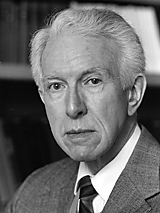
\includegraphics[width=.95\textwidth]{figures/wells.jpg}
  \caption{Rulon Wells}
  \label{fig:ch.structuralists.wells}
\end{wrapfigure}
\citet{wells49:automatic} provides what is probably the most
structured and sophisticated discussion of the theoretical problem of
how rules of \isi{alternation} interact with one another. {\Wells} begins by
noting (citing \citealt{harris42:alternants}) that many morphemes have
more than one phonemic form or alternant, and the problem to be
addressed is how to describe the patterns of \isi{alternation} these
display. Following \citet[211]{bloomfield:lg}, ``[when] the
distribution of the \ldots\ alternants is is regulated according to a
linguistically recognizable characteristic of the accompanying forms,
we say that the \isi{alternation} is \textsc{regular}. [When] \ldots\ the
deciding characteristic of the accompanying forms is phonemic \ldots,
we say that the \isi{alternation} is \textsc{automatic}.'' The goal of the
paper is to characterize the varieties of these automatic
alternations, and to ``produce the most efficient body of statements
from which all the automatic alternations can be deduced'' (p. 101). 

He notes first that ``[i]n general, one of two alternating forms is
predictable from the other'' but not \emph{vice versa}. As a result,
one alternant can be labeled as the ``basic'' alternant, and the
other(s) as ``derived''. Where alternant \emph{A} is basic and
\emph{B} derived, it is common to speak of ``changing'' \emph{A} to
\emph{B} in an appropriate environment, but he is clear that the notion
of ``change'' here is simply a metaphor. It cannot be interpreted as
describing \isi{historical change} (a notion he dismisses repeatedly in the
paper), or as anything other than a mode of description: ``All that is
necessary is to state the morphs of each morpheme and the respective
environments in which they occur'' (p. 102).

Against this background, he proceeds to define four basic sorts of
\isi{automatic alternation}, in formally explicit fashion, in terms of two
independent differences. Essentially, \emph{wide} alternations are
ones in which the environment crucially involves morphological
complexity (i.e., a boundary of some sort), while \emph{narrow}
alternations are also enforced within a single morpheme.\footnote{The
  difference here is similar to that between rules that are or are not
  subject to something like the ``Alternation Condition'' of
  \citealt{kiparsky:3dimensions} or its refinement as a restriction to
  ``derived environments''.} Cross-classifying with this is the
distinction between \emph{static} alternations, in which the
environment for the appearance of a given alternant is stated in terms
of the (surface) phonemic form of the material in its environment, and
\emph{dynamic} alternations, in which the environment for the
appearance of a given alternant is stated in terms of the \emph{basic}
form(s) of the material in the environment. Dynamic alternations in
this sense are similar to those discussed above in which {\Sapir} and
{\Harris} allow rules to have access to basic and not (only) derived
forms.

He observes that the choice of one or another of the four types of
description yields different results, or in some cases the same result
but for different reasons. He notes that the dynamic mode of
description is commonly preferred, but that the reason for this is
simply that most linguists of the time had a background in historical
studies, and the dynamic account is closer to that than is the
static. Since synchronic description does not in any way involve
history, however, this advantage is quite spurious, and indeed has the
disadvantage that a \isi{basic form} must be established for every morpheme,
a condition that may be difficult or impossible to meet in some cases.

An additional complication in each case is the possibility of
describing reciprocally conditioned \isi{variation} simultaneously or in
step-wise fashion, one morpheme at a time. Here too, however, the
notion of sequence is purely a descriptive device rather than an
essential property of the \isi{alternation}. He also considers, at the end
of the paper, the possibility that an \isi{alternation} might be described
in a way involving a fictive ``evanescent'' intermediate form: a
representation produced by an initial interpretation of the basic
forms of the morphemes involved, but not actually occurring, being
necessarily subject to further modification by other patterns, to
yield the observed phonemic form. Although he raises this
possibility, he does not develop it at all, and seems clearly to
deprecate it.

The rigor of {\Wells}'s paper provided a potential framework for the
description of substantial parts of the \isi{morphophonemics} of particular
languages, but aside from occasional citations as a refinement of
{\Bloomfield}'s original notion of an \isi{automatic alternation}, there is no
evidence that this framework was actually appealed to in concrete
descriptions, and it is notable that it was not included in
\posscitet{joos57:readings} collection of essential works. The very
extent to which the paper was generally ignored by other linguists at
the time probably illustrates well just how marginal such concerns
were in the context of American structuralist theoretical discussion.

Within American structuralist theory, \isi{morphophonemics} had no real
status other than as a `technique' for describing in a compact way the
sets of allomorphs belonging to individual morphemes. Morphophonemics
deals with \isi{regularities} in the relations between forms, but since only
the forms themselves are directly observable, in terms of the American
structuralists' limited view of the nature of language, only the
phonemic forms are `real'. Regularities are not facts of the same
order, to be accorded the same status in the grammar: rather they are
something that can be found by the linguist in the relation between
forms. Of course, it is incumbent on the linguist to describe these
relations, but how to go about that is the scientist's own business
and not a matter of linguistic fact.

\citet{goldsmith08:genphon.in.40s} argues, to the contrary, that
\posscitet{wells49:automatic} account of automatic alternations was
intended to advocate a model close to that of 1960s Generative
Phonology, in which (underlying) base forms are converted by an
ordered sequence of \isi{morphophonemic rules} (possibly passing through
`fictive' intermediate stages which are not identical either with base
or surface forms) into surface phonemic forms. This interpretation
seems forced to the present writer: although much of the apparatus
necessary to such an account is developed in {\Wells}'s descriptions, the
notion that he thought such a picture was appropriate and an actual
part of the language, as opposed to one in which only the surface
phonemic forms are `real' and the rest artifacts of a convenient mode
of description, does not carry conviction.  His view of what is
essential to the language, as opposed to a description that the
linguist chooses as the most efficient, seems well expressed by the
quote above that ``[a]ll that is necessary is to state the morphs of
each morpheme and the respective environments in which they occur''
\citep[102]{wells49:automatic}.

It is true that {\Bloomfield} (among others) discussed the existence of
alternative descriptions of the same sets of facts, and proposed
choices among these. More specifically, {\Bloomfield} in several places
urges that the analyst should always choose the `simplest' available
solution. In the light of subsequent linguistic theory, one might
therefore be tempted to attribute to him a notion of evaluation
applicable to the comparison of grammatical descriptions, in the
domain of \isi{morphophonemics} as well as elsewhere; but this would fairly
clearly be an error. When {\Bloomfield} talks about one description as
`simpler' than another, he does not mean this in the technical sense
later given to it in \isi{generative grammar} (chapter~\ref{ch.genphon}), but
simply in the pre-systematic sense that one description might be
shorter, less complicated, less redundant, neater, etc. than
another. Naturally, linguists should strive to maximize readability,
and also conciseness. Beyond this, however, and as a question of a
`correct' linguistic analysis, any description was potentially correct
if it got the forms right, and presented an accurate account of the
phonemic, morphemic, etc. systems of the language.

For the American structuralists, as for {\Bloomfield}, a language was
basically a hierarchy of inventories: an inventory of phonemes, which
could be concatenated to form \isi{morpheme alternants}; an inventory of
morphemes, which could be combined to form words and syntactic
constructions which themselves formed further inventories. A
description of a language was fundamentally a definition and
enumeration of the elements that made up these inventories.

Only when this conception was replaced by the notion that a language
is a structured cognitive system was it possible to take seriously the
idea that a description had to comprehend something other than the set
of forms (at various \isi{levels} of analysis). In describing such a
cognitive system, not only the forms but also the rules which express
\isi{regular} relations among them (and further, the principles which
determine the interpretation and application of the rules) correspond
to something `real'. In those terms, it is possible to raise the issue
of whether a particular description, or a particular format for
descriptions in general, is right or wrong. For American
structuralists, however, \isi{morphophonemics} fell entirely into the area
of `\isi{regularities}' rather than that of `items', and since their
principles excluded such facts from phonemics, this aspect of
\isi{linguistic description} occupied only the non-systematic status of a
descriptive technique that was not really part of the language itself.

%%% Local Variables: 
%%% mode: latex
%%% TeX-master: "/Users/sra/Dropbox/Docs/Books/P20C_2/LSP/main.tex"
%%% End: 
